\chapter{Diseño e implementación}

En este capítulo se documenta el diseño e implementación que se ha realizado para dar lugar a la aplicación final. Como bien se explica en el capítulo dedicado a la arquitectura, se ha seguido una división por subsistemas por lo que la mejor aproximación para separar ahora los múltiples diagramas de clases es hacerlo por paquetes, asociados cada uno de ellos a un subsistema. Además se generarán una serie de paquetes que contienen una serie de funcionalidades adicionales utilizadas por los otros.

\bigskip

Se empezará por la documentación asociada a los paquetes relacionados con el motor del videojuego en sí mismo para luego seguir con el subsistema de la lógica de la aplicación que contendrá la implementación del agente. Luego se muestran los diagramas de interacción que relacionan las clases antes definidas con los casos de uso en los que participan. Finalmente se mostrará como se llegó al diseño de la interfaz gráfica de la aplicación.Además, se ha hecho uso de un \textbf{código de colores} que permite una comprensión más rápida de cada uno de los diagramas:

\begin{itemize}
	\item \textbf{Verde}: Identifica las clases protagonistas o principales de cada diagrama.
	\item \textbf{Morado}: Identifica las clases que ayudan a las principales a realizar la función que se les requiere, estas clases \textbf{pertenecen} al paquete/diagrama que se está mostrando.
	\item \textbf{Amarillo}: Identifica las clases que son necesarias para llevar a cabo las funcionalidades del paquete/subsistema pero que \textbf{no pertenecen} al mismo.
	\item \textbf{Azul}: Identifica las clases, estructuras o enumeraciones que representan contenedores de datos sin funcionalidades complejas.
\end{itemize}

\section{Diagramas de clases}

Para facilitar la comprensión de la estructura de esta sección la misma está ordenada de la siguiente forma:

\begin{enumerate}
	\item Primero se explicará la estructura asociada al bus de mensajes.
	\item Luego se mostrará la estructura genérica de la aplicación con todos los subsistemas.
	\item Se explicarán los subsistemas individualmente.
	\item Brevemente, se mencionarán algunas clases adicionales.
	\item Finalmente se mostrarán los diagramas de cada una de las escenas.
\end{enumerate}

En los apartados que siguen se añadirá una breve explicación asociada a cada diagrama para favorecer su comprensión. 

\subsection{Bus de mensajes}

\begin{figure}
	\centerline{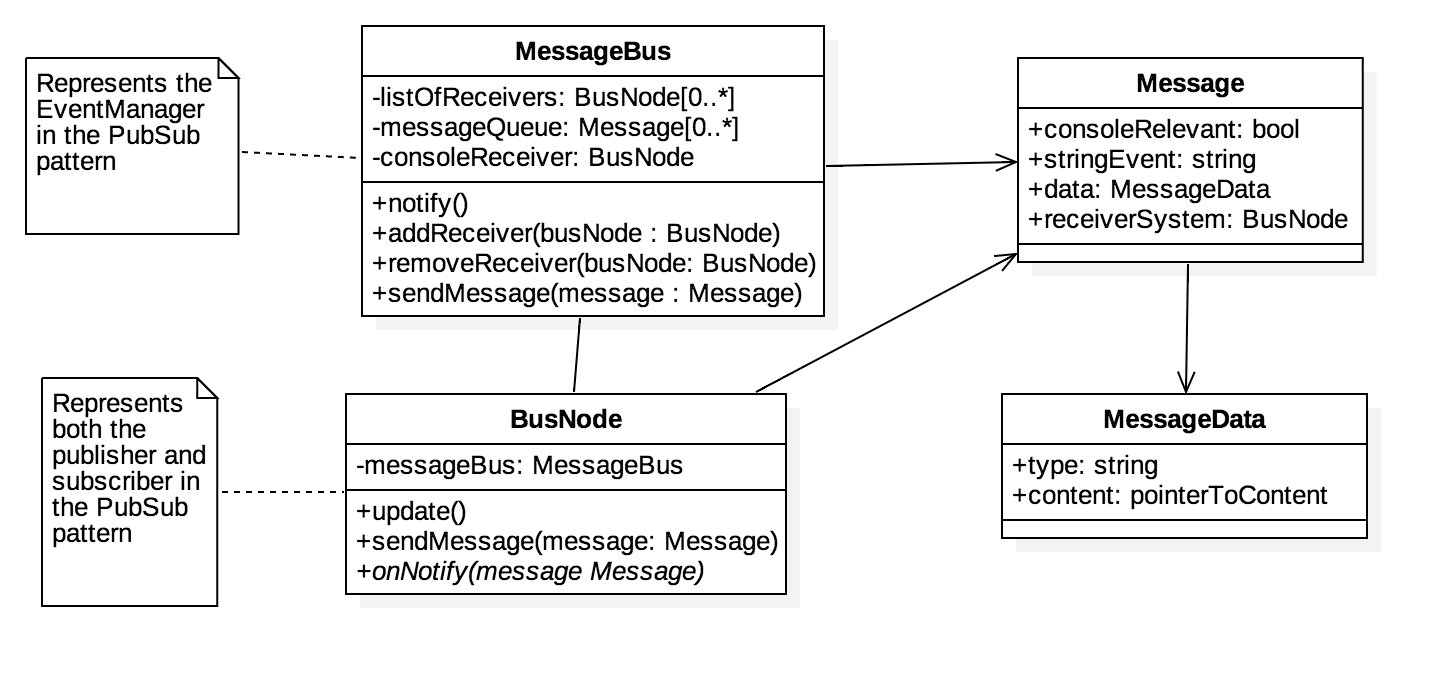
\includegraphics[width=15cm]{otros/UML/png/alld/png/messaging__diagramaDeClases_messaging_11.png}}
	\caption{Diagrama de clases del bus de mensajes}
	\label{class:messageBus}
\end{figure}

En la figura \ref{class:messageBus} se encuentra el diagrama de clases del bus de mensajes, en el mismo se vé implementada una modificación del patrón \textit{PubSub} (mostrado en la figura \ref{pat:pubsub}) en la cual la clase \textbf{\textit{BusNode}} representa tanto a los publicadores como a los subscriptores. Dicha clase es la encargada de encapsular las funcionalidades asociadas a enviar y recibir mensajes por parte de cada subsistema.

\bigskip

Por otra parte, la clase \textbf{\textit{MessageBus}} es la que representa el \textit{EventManager} del patrón \textit{PubSub}. La misma es la encargada de almacenar los mensajes y enviarlos a todas las instancias de \textit{BusNode} que lo requieran.

\bigskip

Finalmente, se ven las clases \textbf{\textit{Message}} y \textbf{\textit{MessageData}} que representan los mensajes que se envía y su contenido.

\subsection{Aplicación general}

\begin{figure}
	\centerline{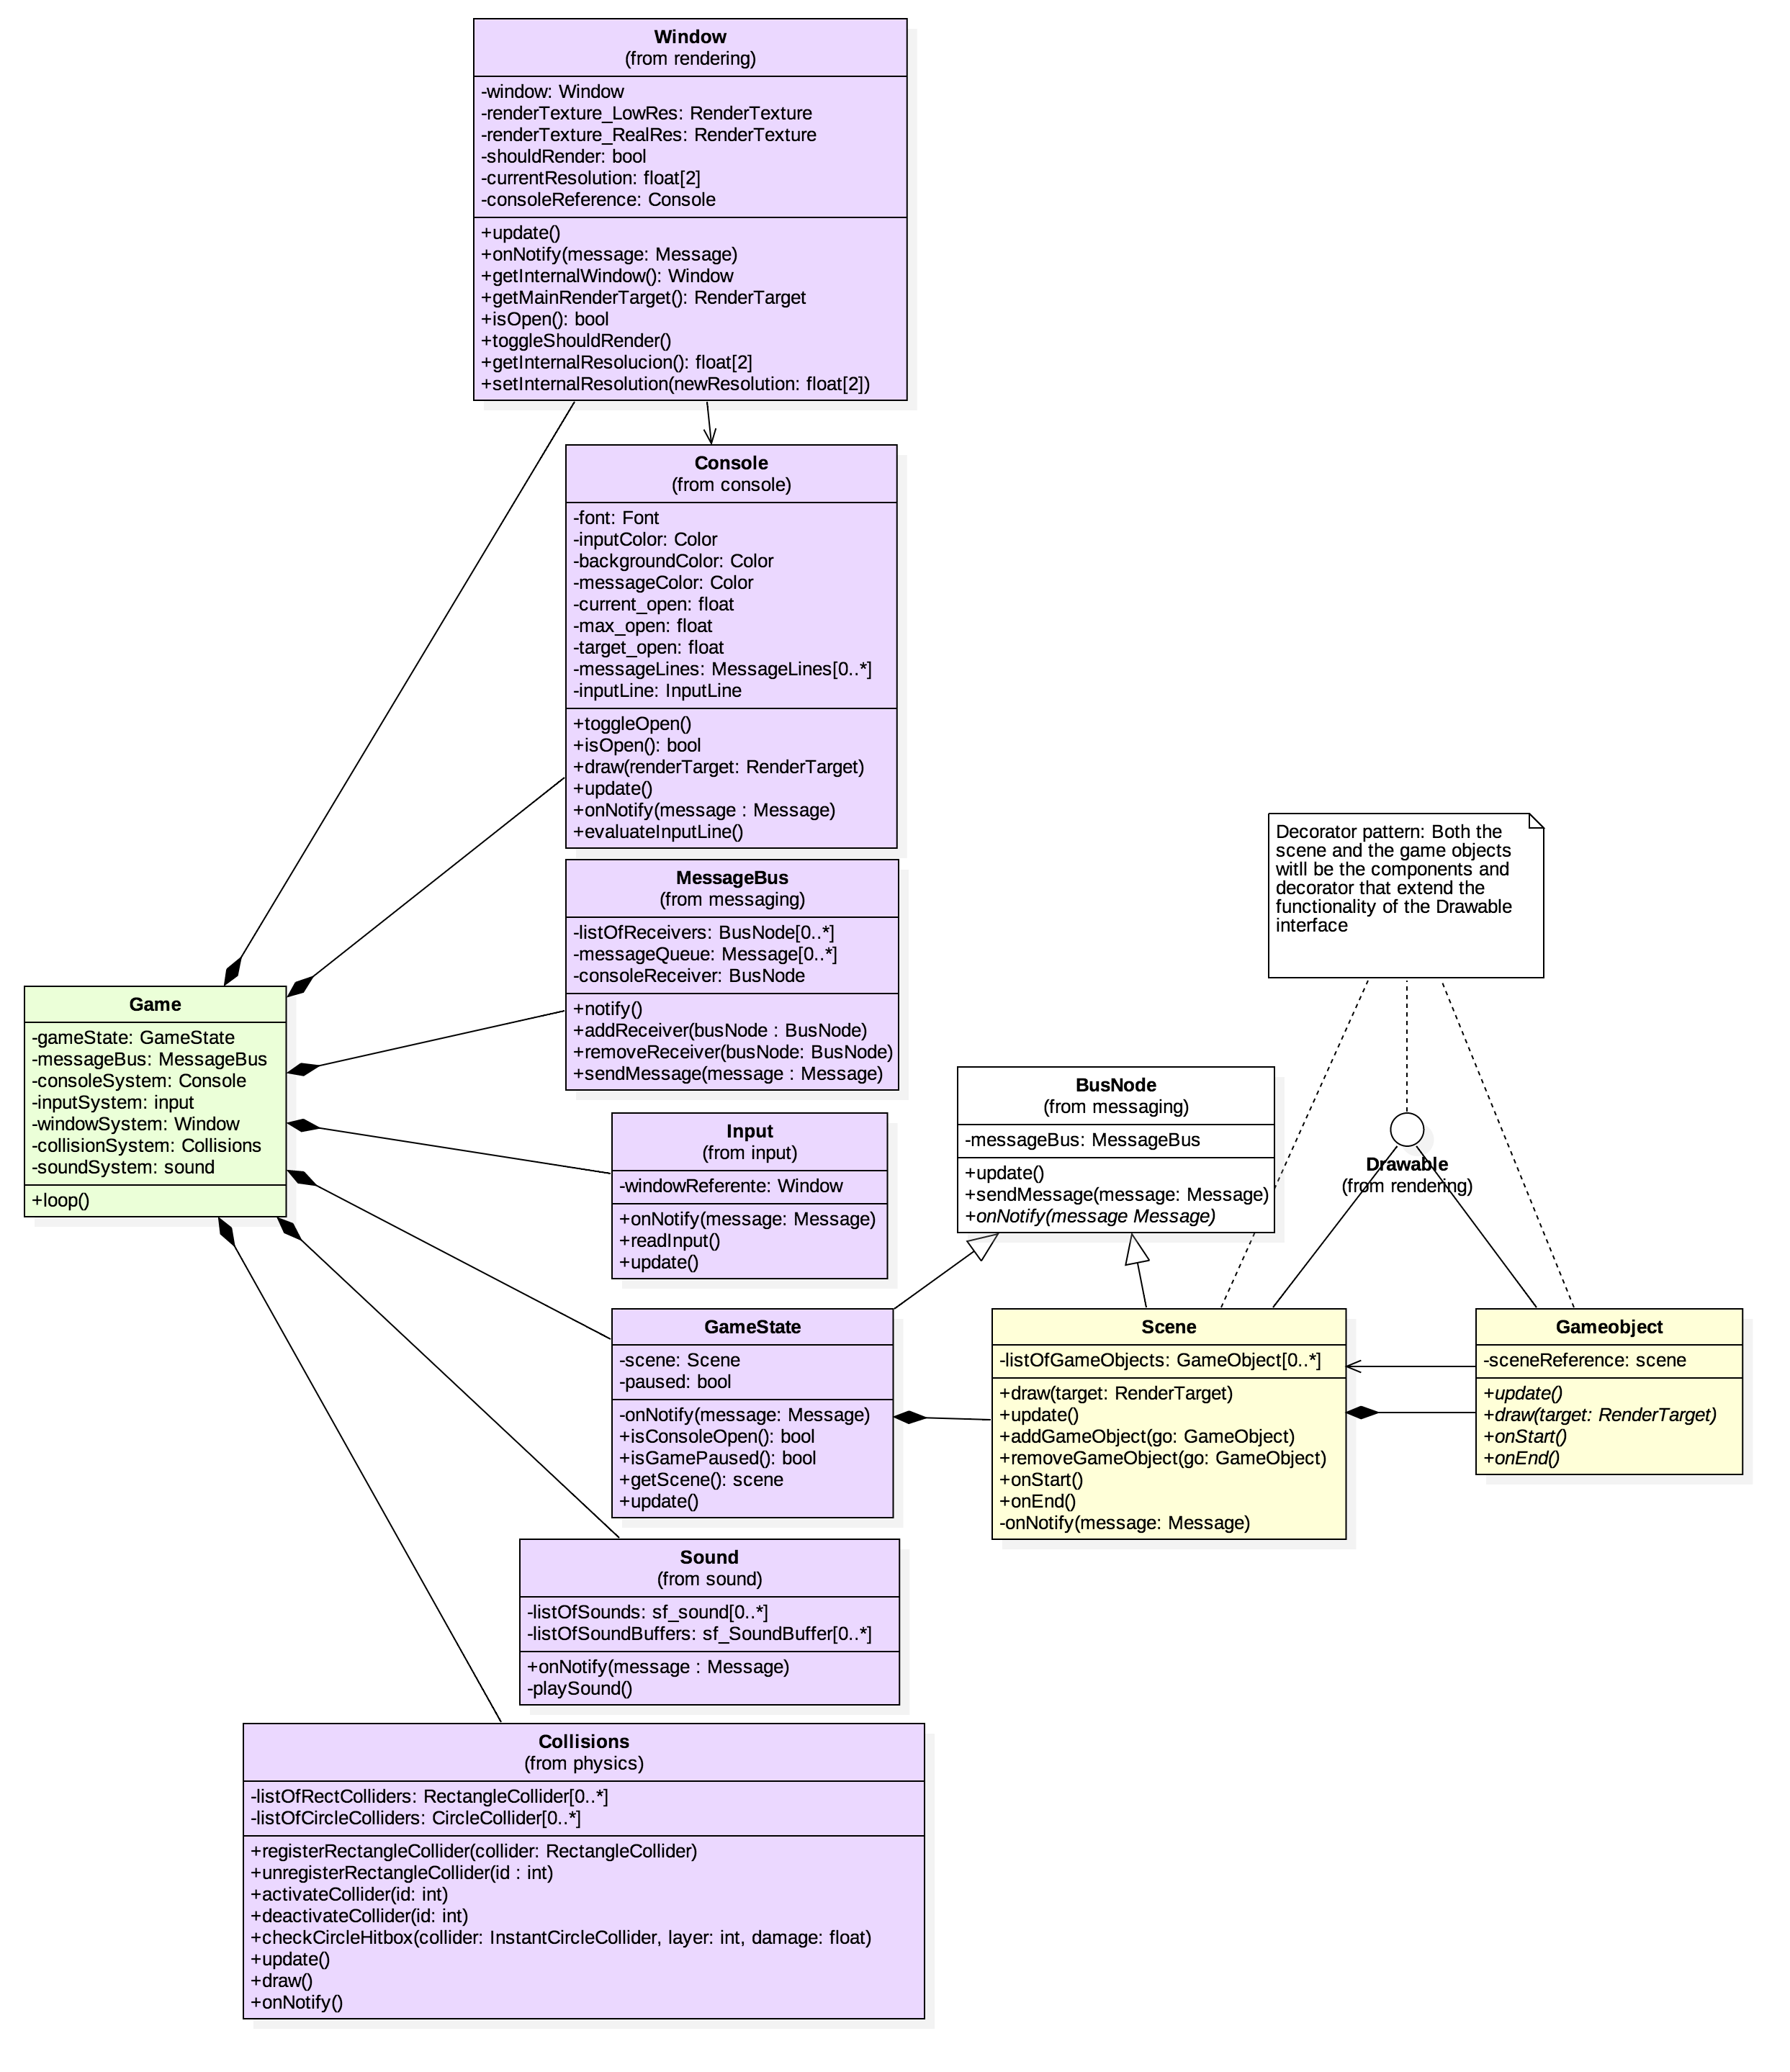
\includegraphics[width=18cm]{otros/UML/png/alld/png/gamelogic__diagramaDeClases_gamelogic_7.png}}
	\caption{Diagrama de clases de la lógica del juego}
	\label{class:gamelogic}
\end{figure}

La figura \ref{class:gamelogic} contiene la lógica del juego mostrada a muy alto nivel. La clase principal es \textbf{\textit{Game}} que es instanciada en el \textit{main} de la aplicación. La misma contiene la función \textit{loop} que simplemente itera por todos los subsistemas, actualizándolos, como se ve en el diagrama de secuencia \ref{sec:general}. 

\bigskip

También se observan las clases asociadas a cada uno de los subsistemas, muy importante es la clase \textbf{\textit{GameState}} que contiene a la escena de la aplicación representada por la clase \textbf{\textit{Scene}}. Aquí podemos ver el patrón \textit{Decorator} (Figura \ref{pat:decorator}) en el cual la escena y los \textit{gameobjects} (representados en la clase \textbf{\textit{GameObject}}) agregan estado y funcionalidad. Cada \textit{gameobject} representa uno de los objetos pertenecientes a la escena desde el punto de vista del juego a alto nivel, esto puede ser un personaje, texto, una barra de vida, un contador de tiempo, etc.


\subsection{Subsistemas}



\begin{figure}
	\centerline{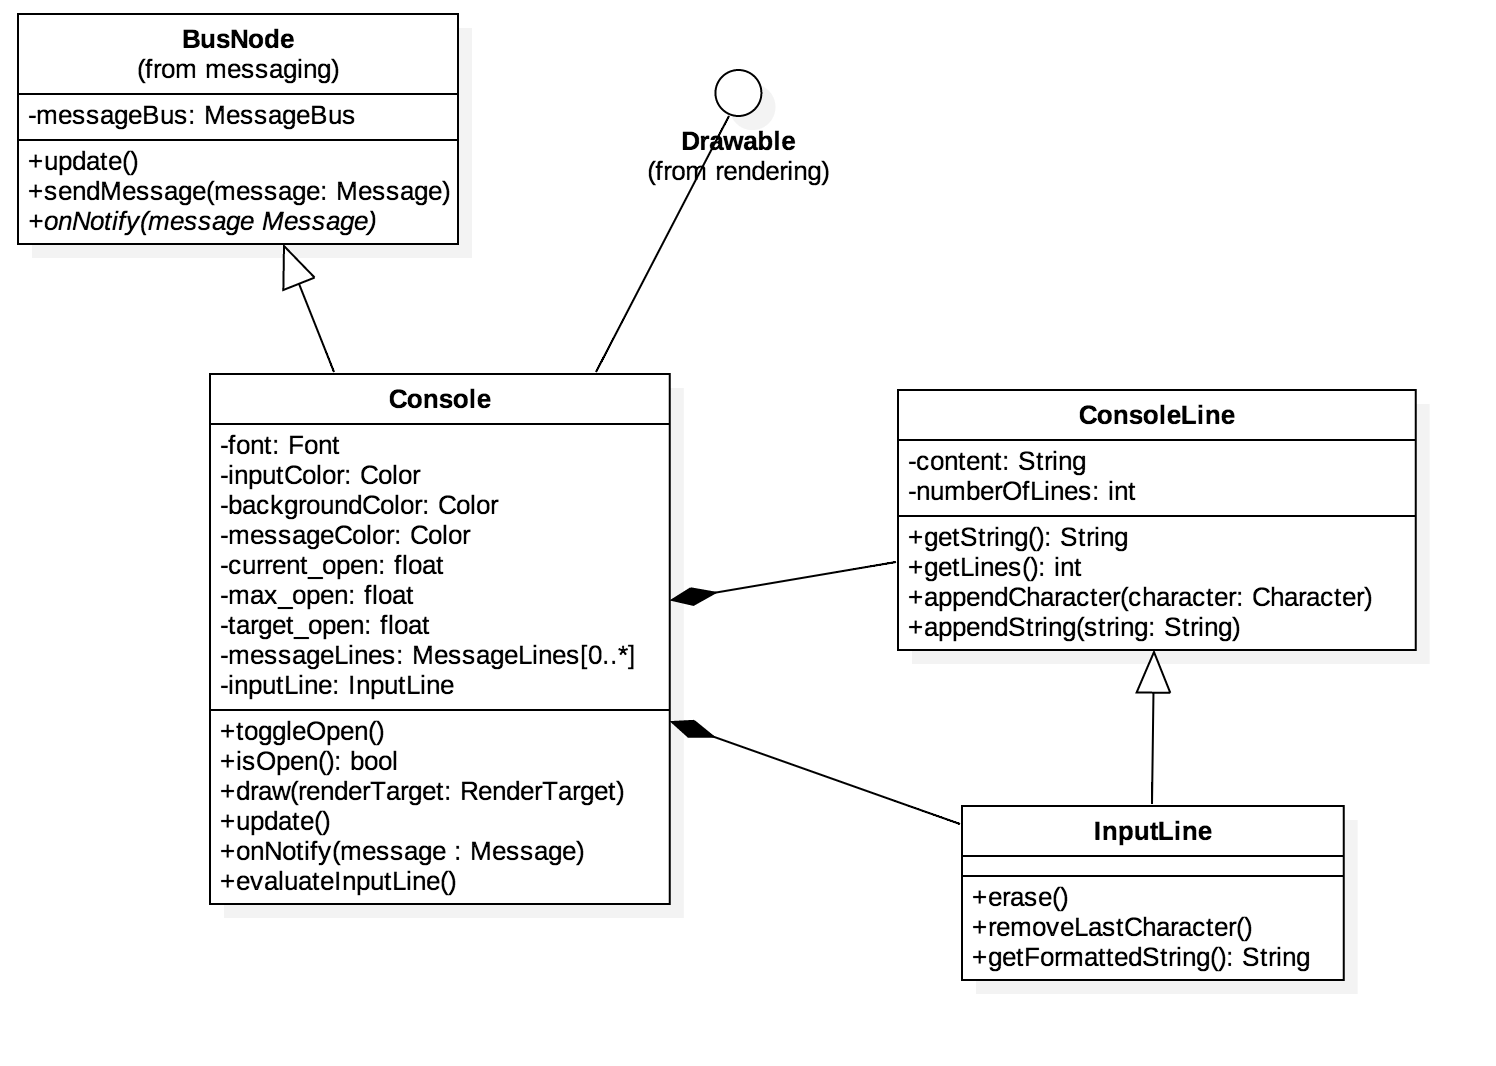
\includegraphics[width=15cm]{otros/UML/png/alld/png/console__diagramaDeClases_console_3.png}}
	\caption{Diagrama de clases del subsistema de consola}
	\label{class:console}
\end{figure}

\begin{figure}
	\centerline{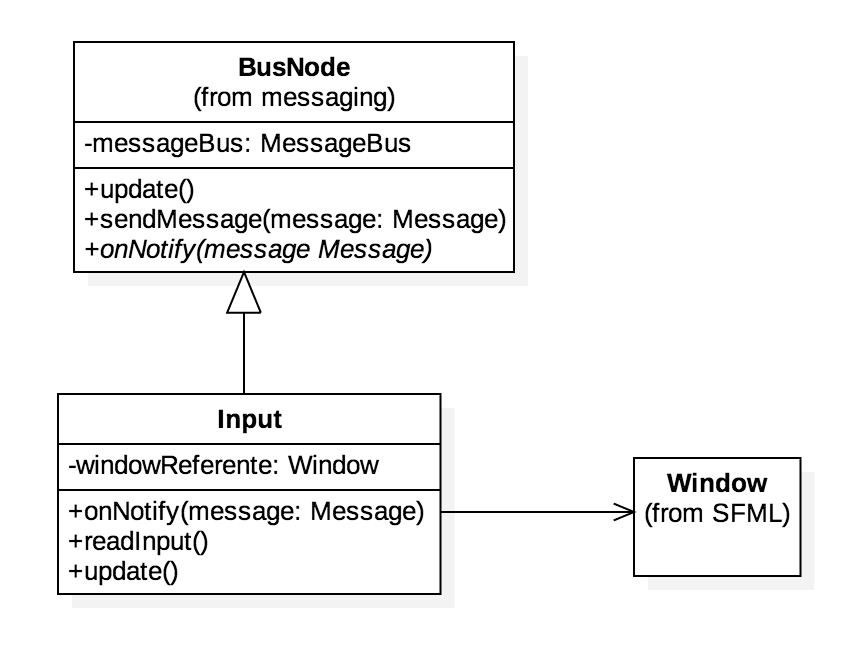
\includegraphics[width=12cm]{otros/UML/png/alld/png/input__diagramaDeClases_input_8.png}}
	\caption{Diagrama de clases del subsistema de entrada}
	\label{class:input}
\end{figure}

\begin{figure}
	\centerline{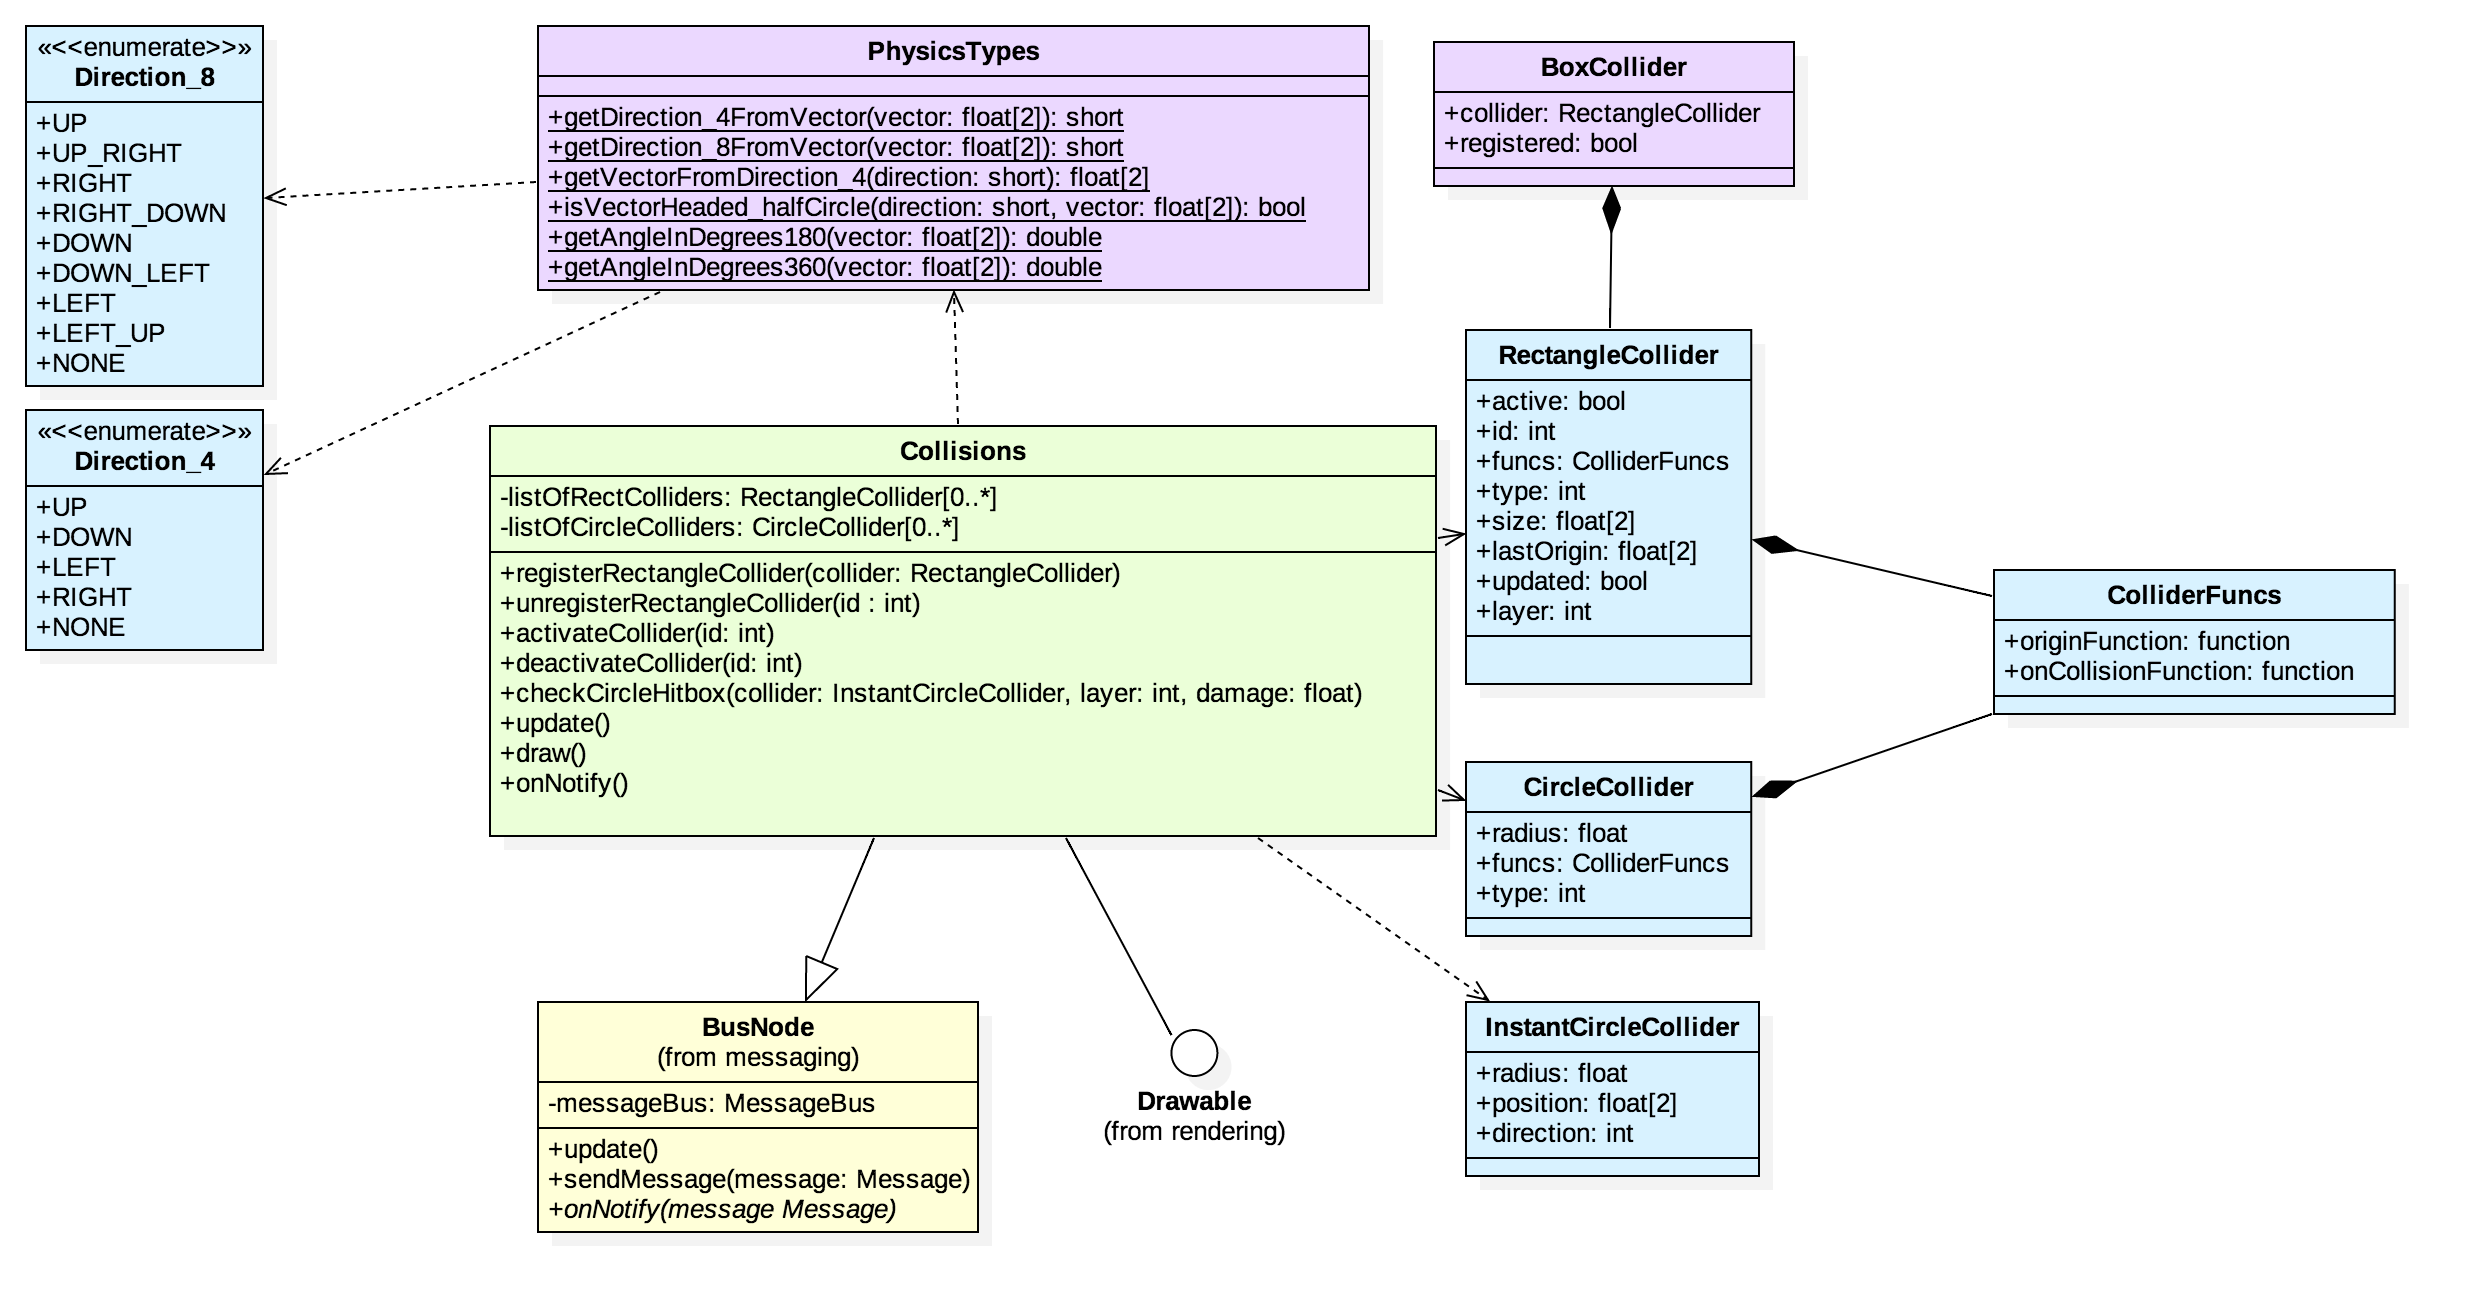
\includegraphics[width=18cm]{otros/UML/png/alld/png/physics__diagramaDeClases_physics_2.png}}
	\caption{Diagrama de clases del subsistema de físicas}
	\label{class:collisions}
\end{figure}

\begin{figure}
	\centerline{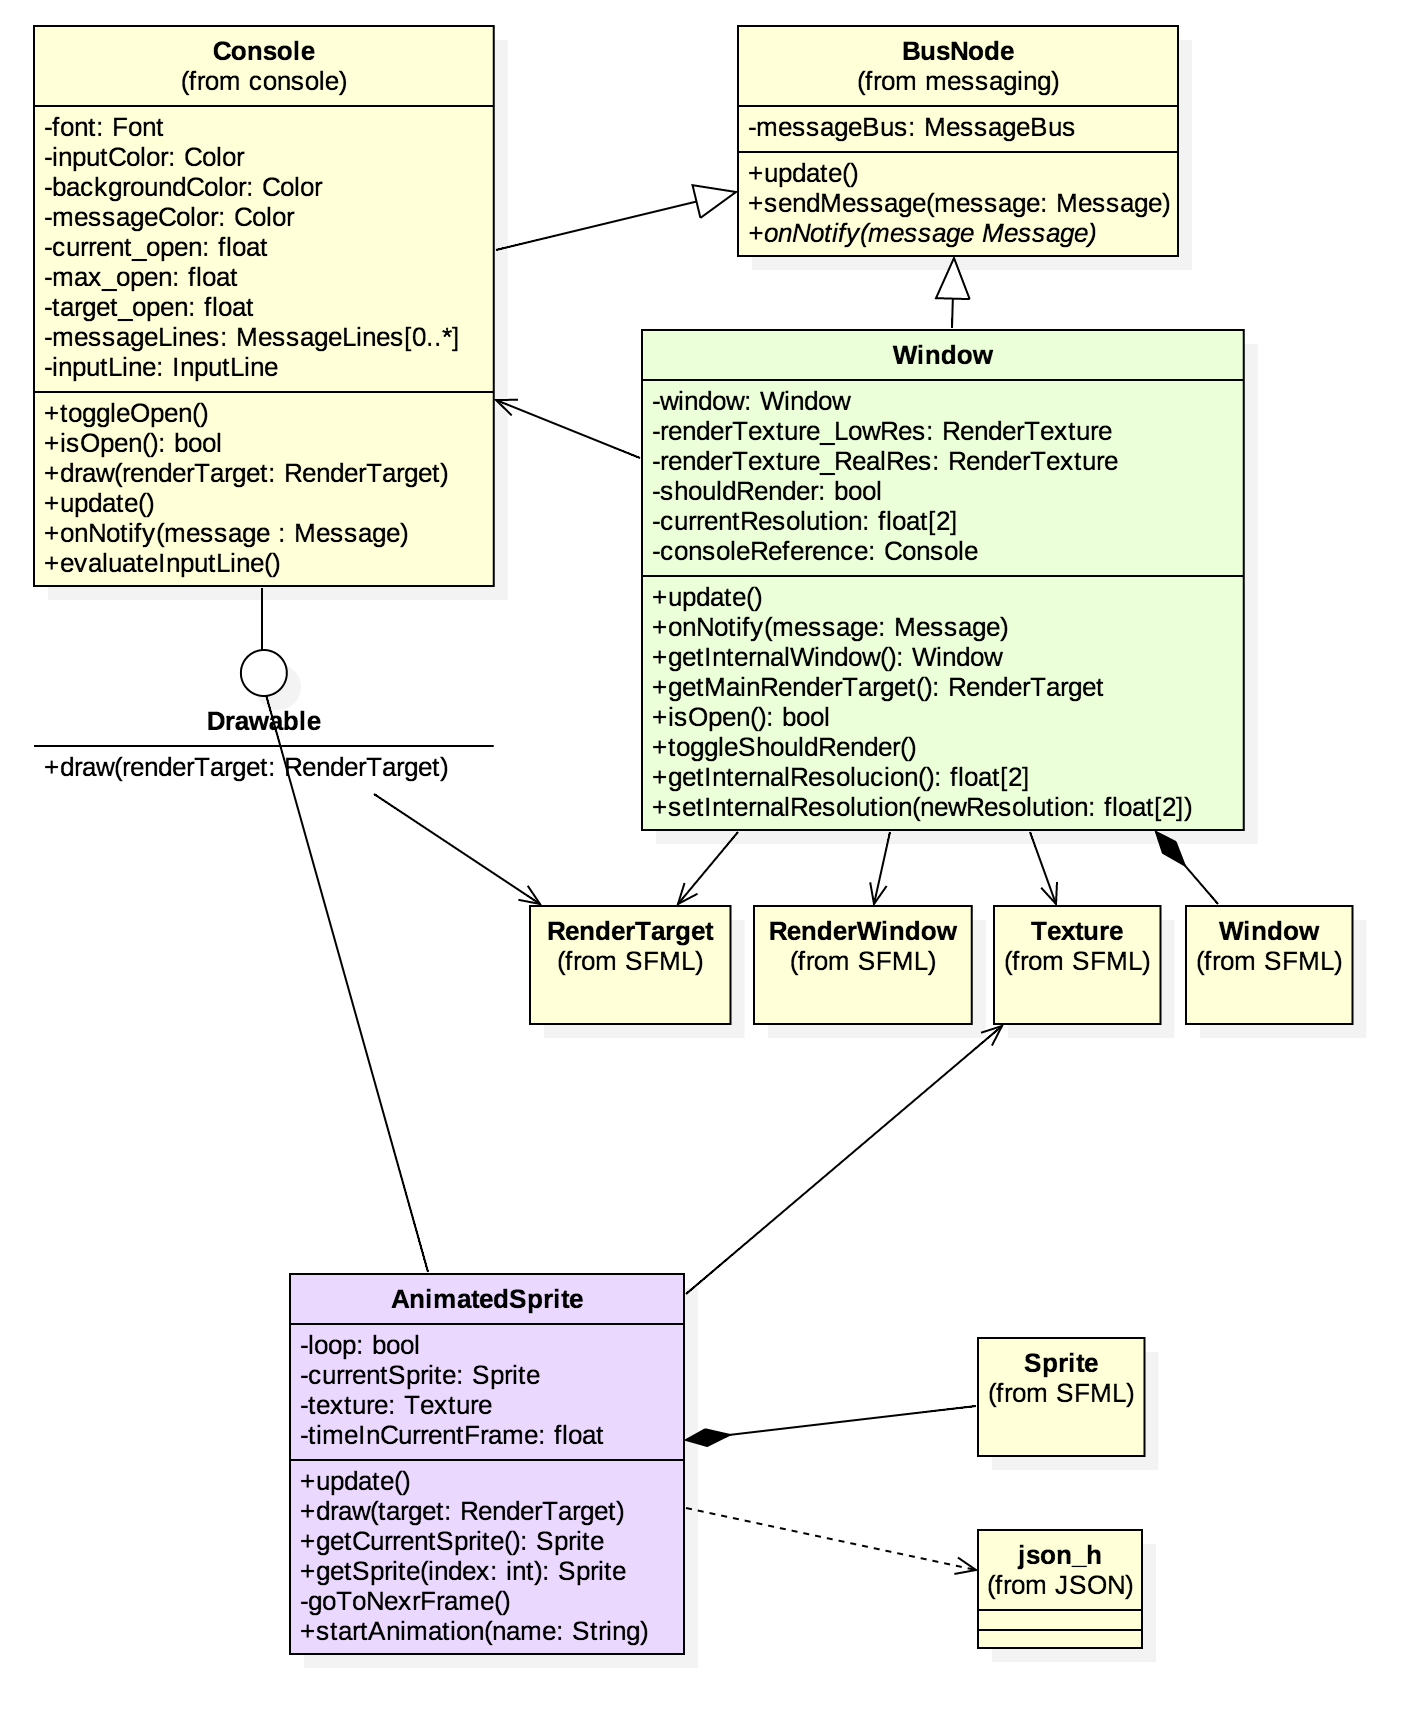
\includegraphics[width=15cm]{otros/UML/png/alld/png/rendering__diagramaDeClases_rendering_9.png}}
	\caption{Diagrama de clases del subsistema de renderizado}
	\label{class:rendering}
\end{figure}


\begin{figure}
	\centerline{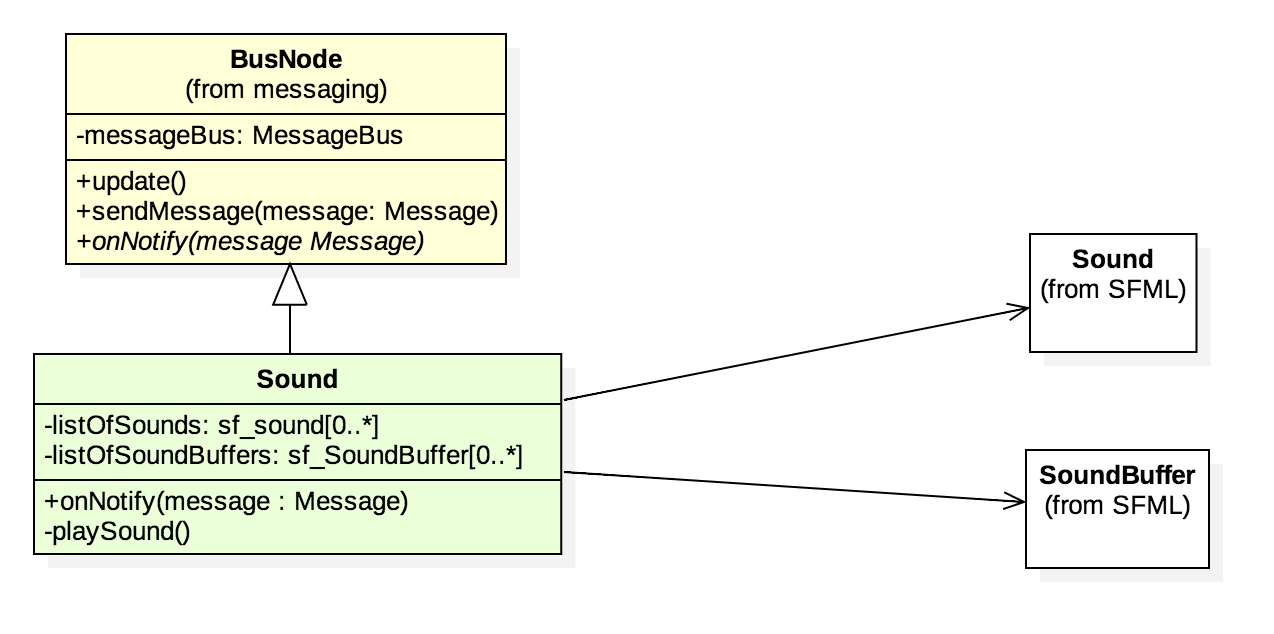
\includegraphics[width=15cm]{otros/UML/png/alld/png/sound__diagramaDeClases_sound_1.png}}
	\caption{Diagrama de clases del subsistema de sonido}
	\label{class:sound}
\end{figure}

\subsection{Otros útiles}

\begin{figure}
	\centerline{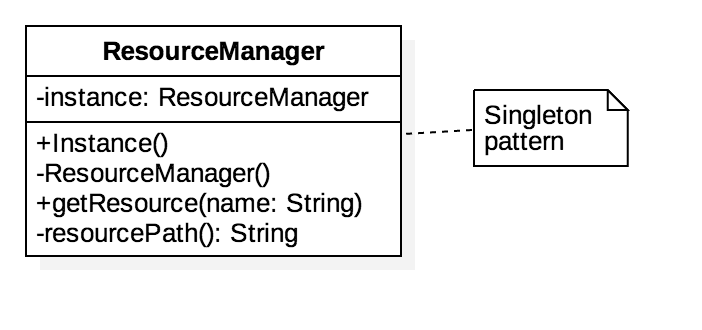
\includegraphics[width=8cm]{otros/UML/png/alld/png/resources__diagramaDeClases_resources_0.png}}
	\caption{Diagrama de clases del paquete de recursos}
	\label{class:resources}
\end{figure}

\begin{figure}
	\centerline{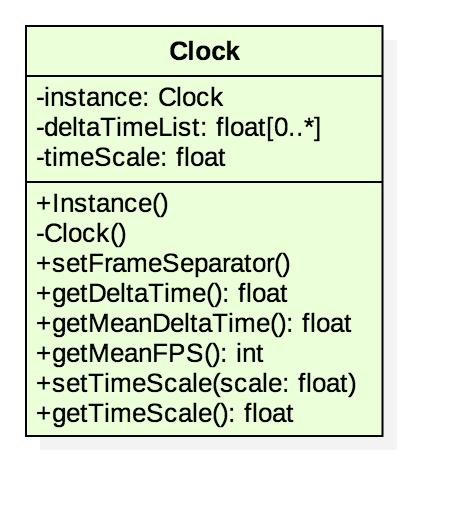
\includegraphics[width=5cm]{otros/UML/png/alld/png/utils__diagramaDeClases_utils_10.png}}
	\caption{Diagrama de clases del paquete de útiles}
	\label{class:utils}
\end{figure}


\subsection{Escenas}

\begin{figure}
	\centerline{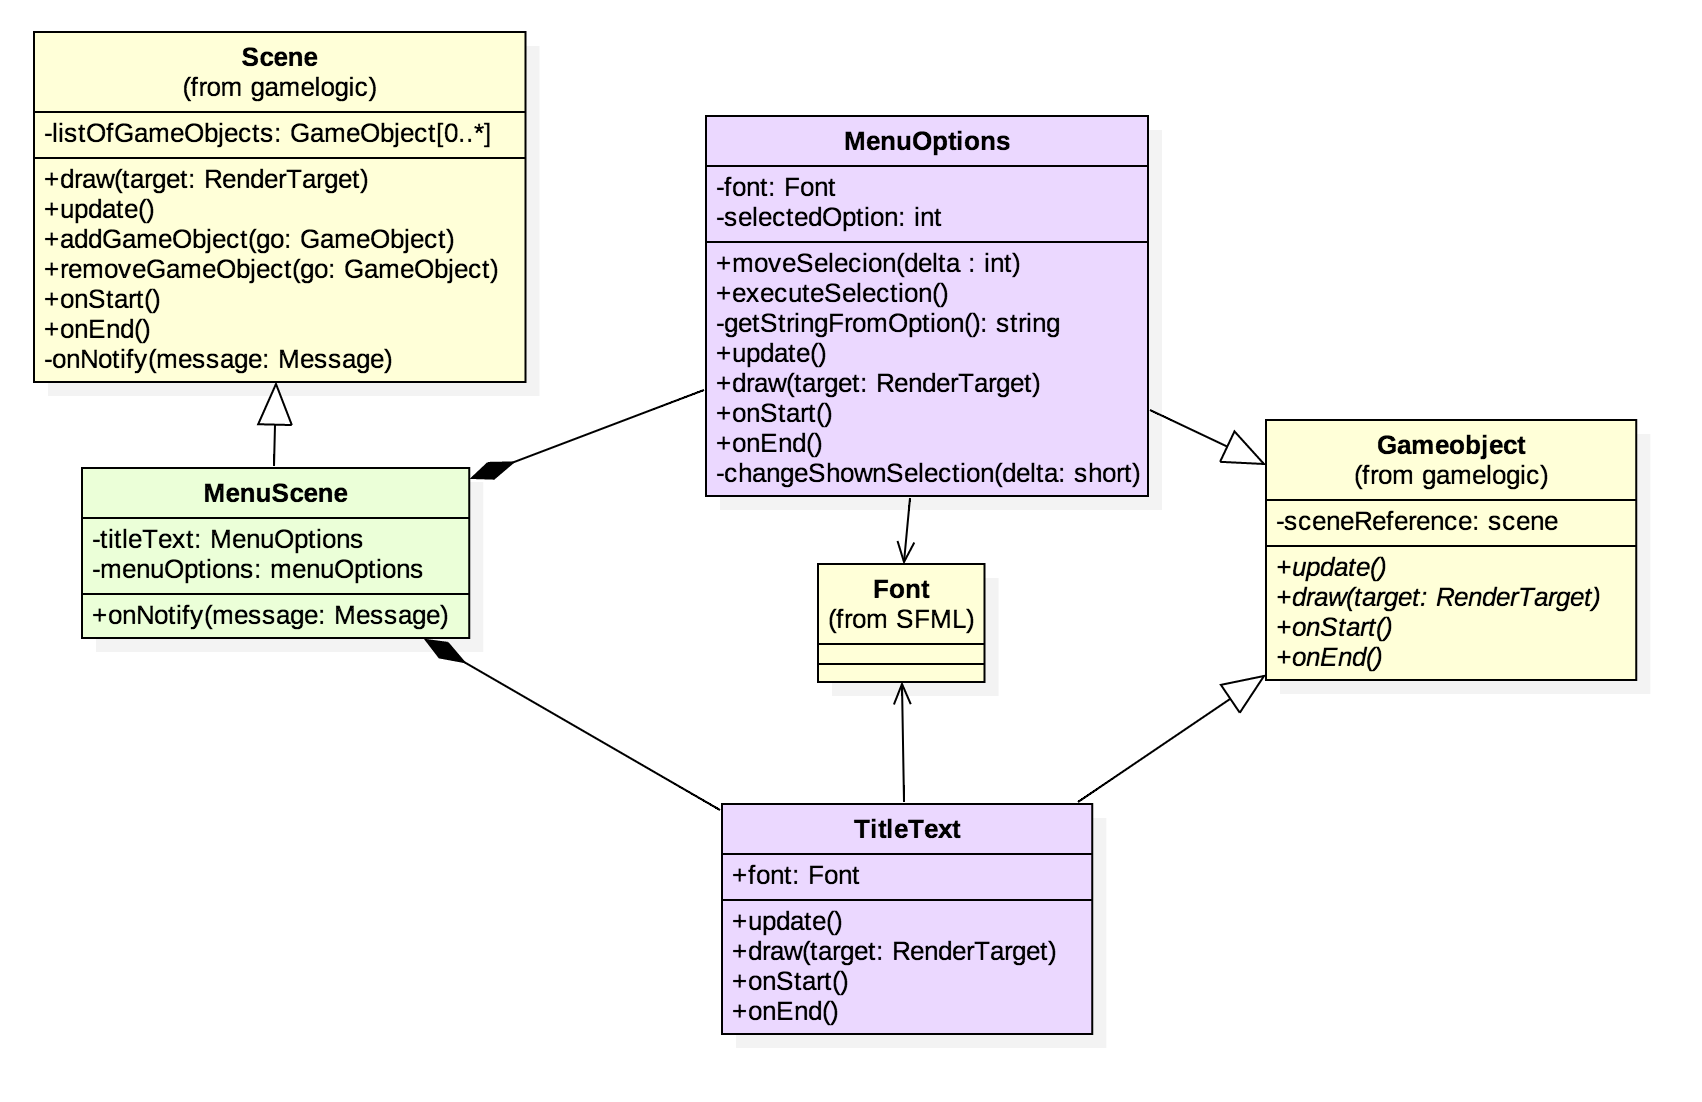
\includegraphics[width=15cm]{otros/UML/png/alld/png/gamelogic__menu__diagramaDeClases_scene_menu_6.png}}
	\caption{Diagrama de clases de la escena del menú}
	\label{class:scene}
\end{figure}

\begin{figure}
	\caption{Diagrama de clases de la escena de juego}
	\hspace*{+1cm}  
	\centerline{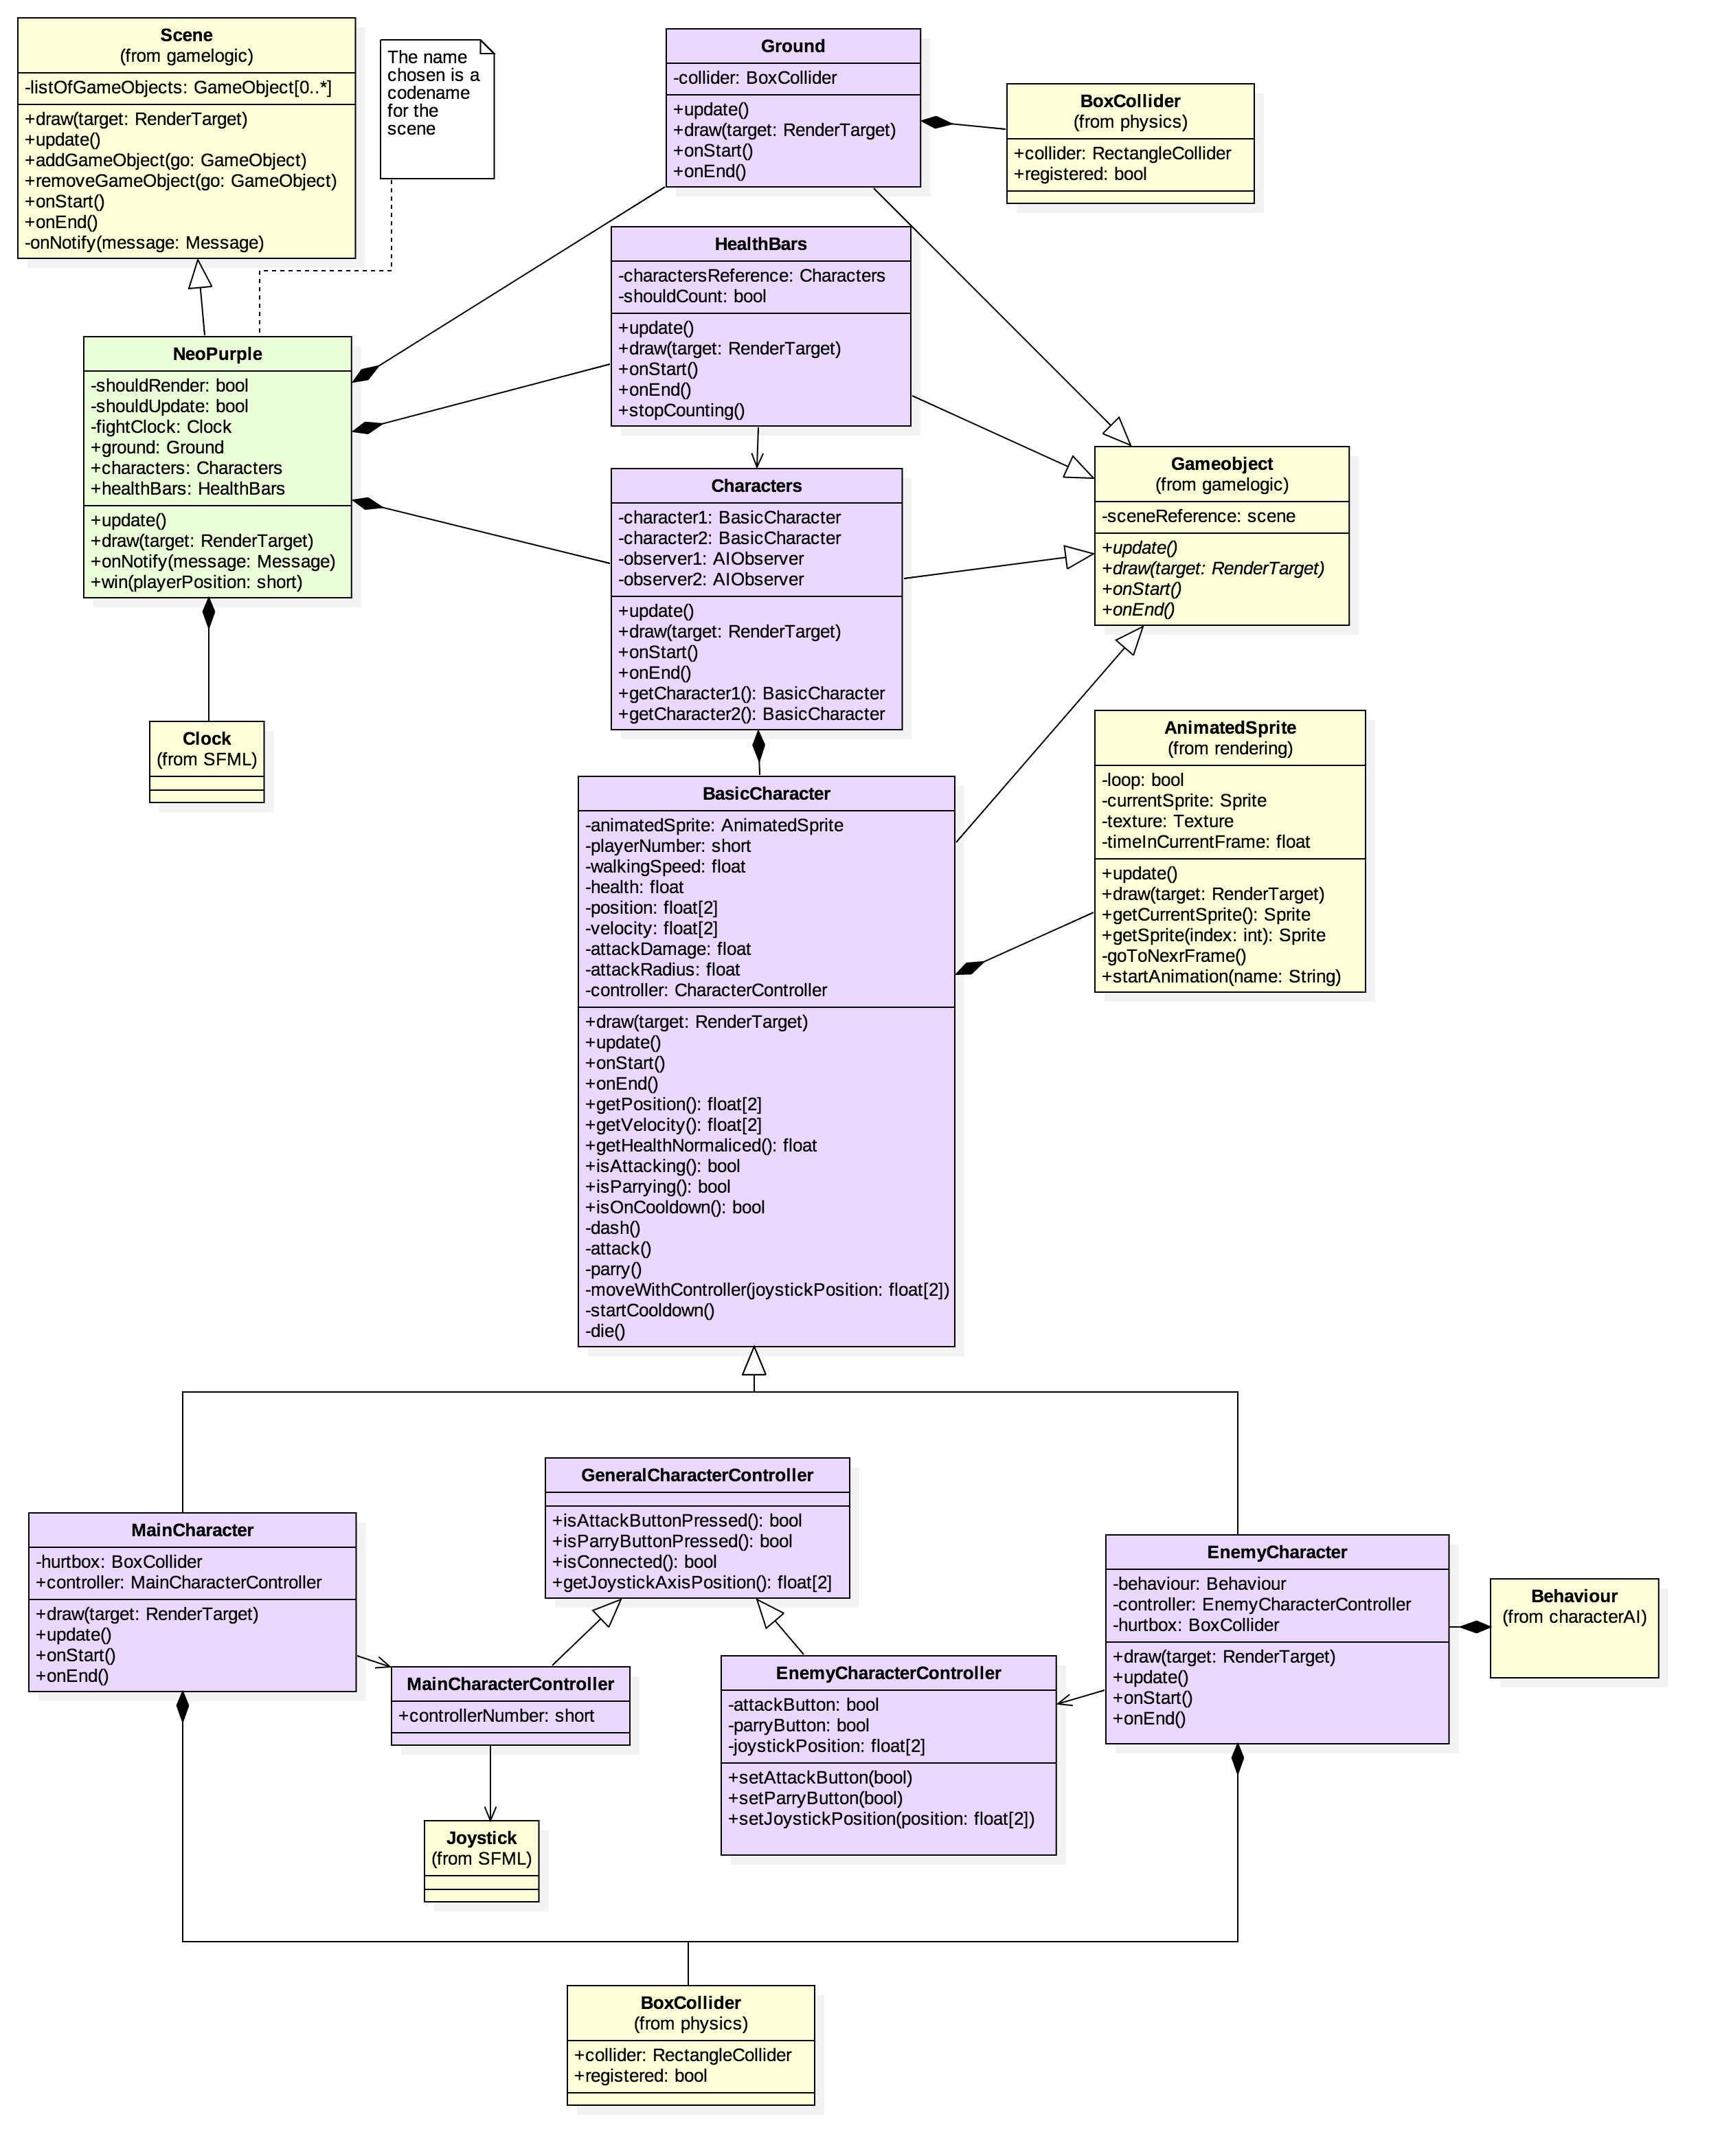
\includegraphics[width=20cm]{otros/UML/png/alld/png/gamelogic__gameplay__diagramaDeClases_scene_gameplay_4.png}}
	\label{class:gameplay}
\end{figure}

\clearpage
\begin{landscape}
\begin{figure}
	\begin{adjustwidth}{-3cm}{}
		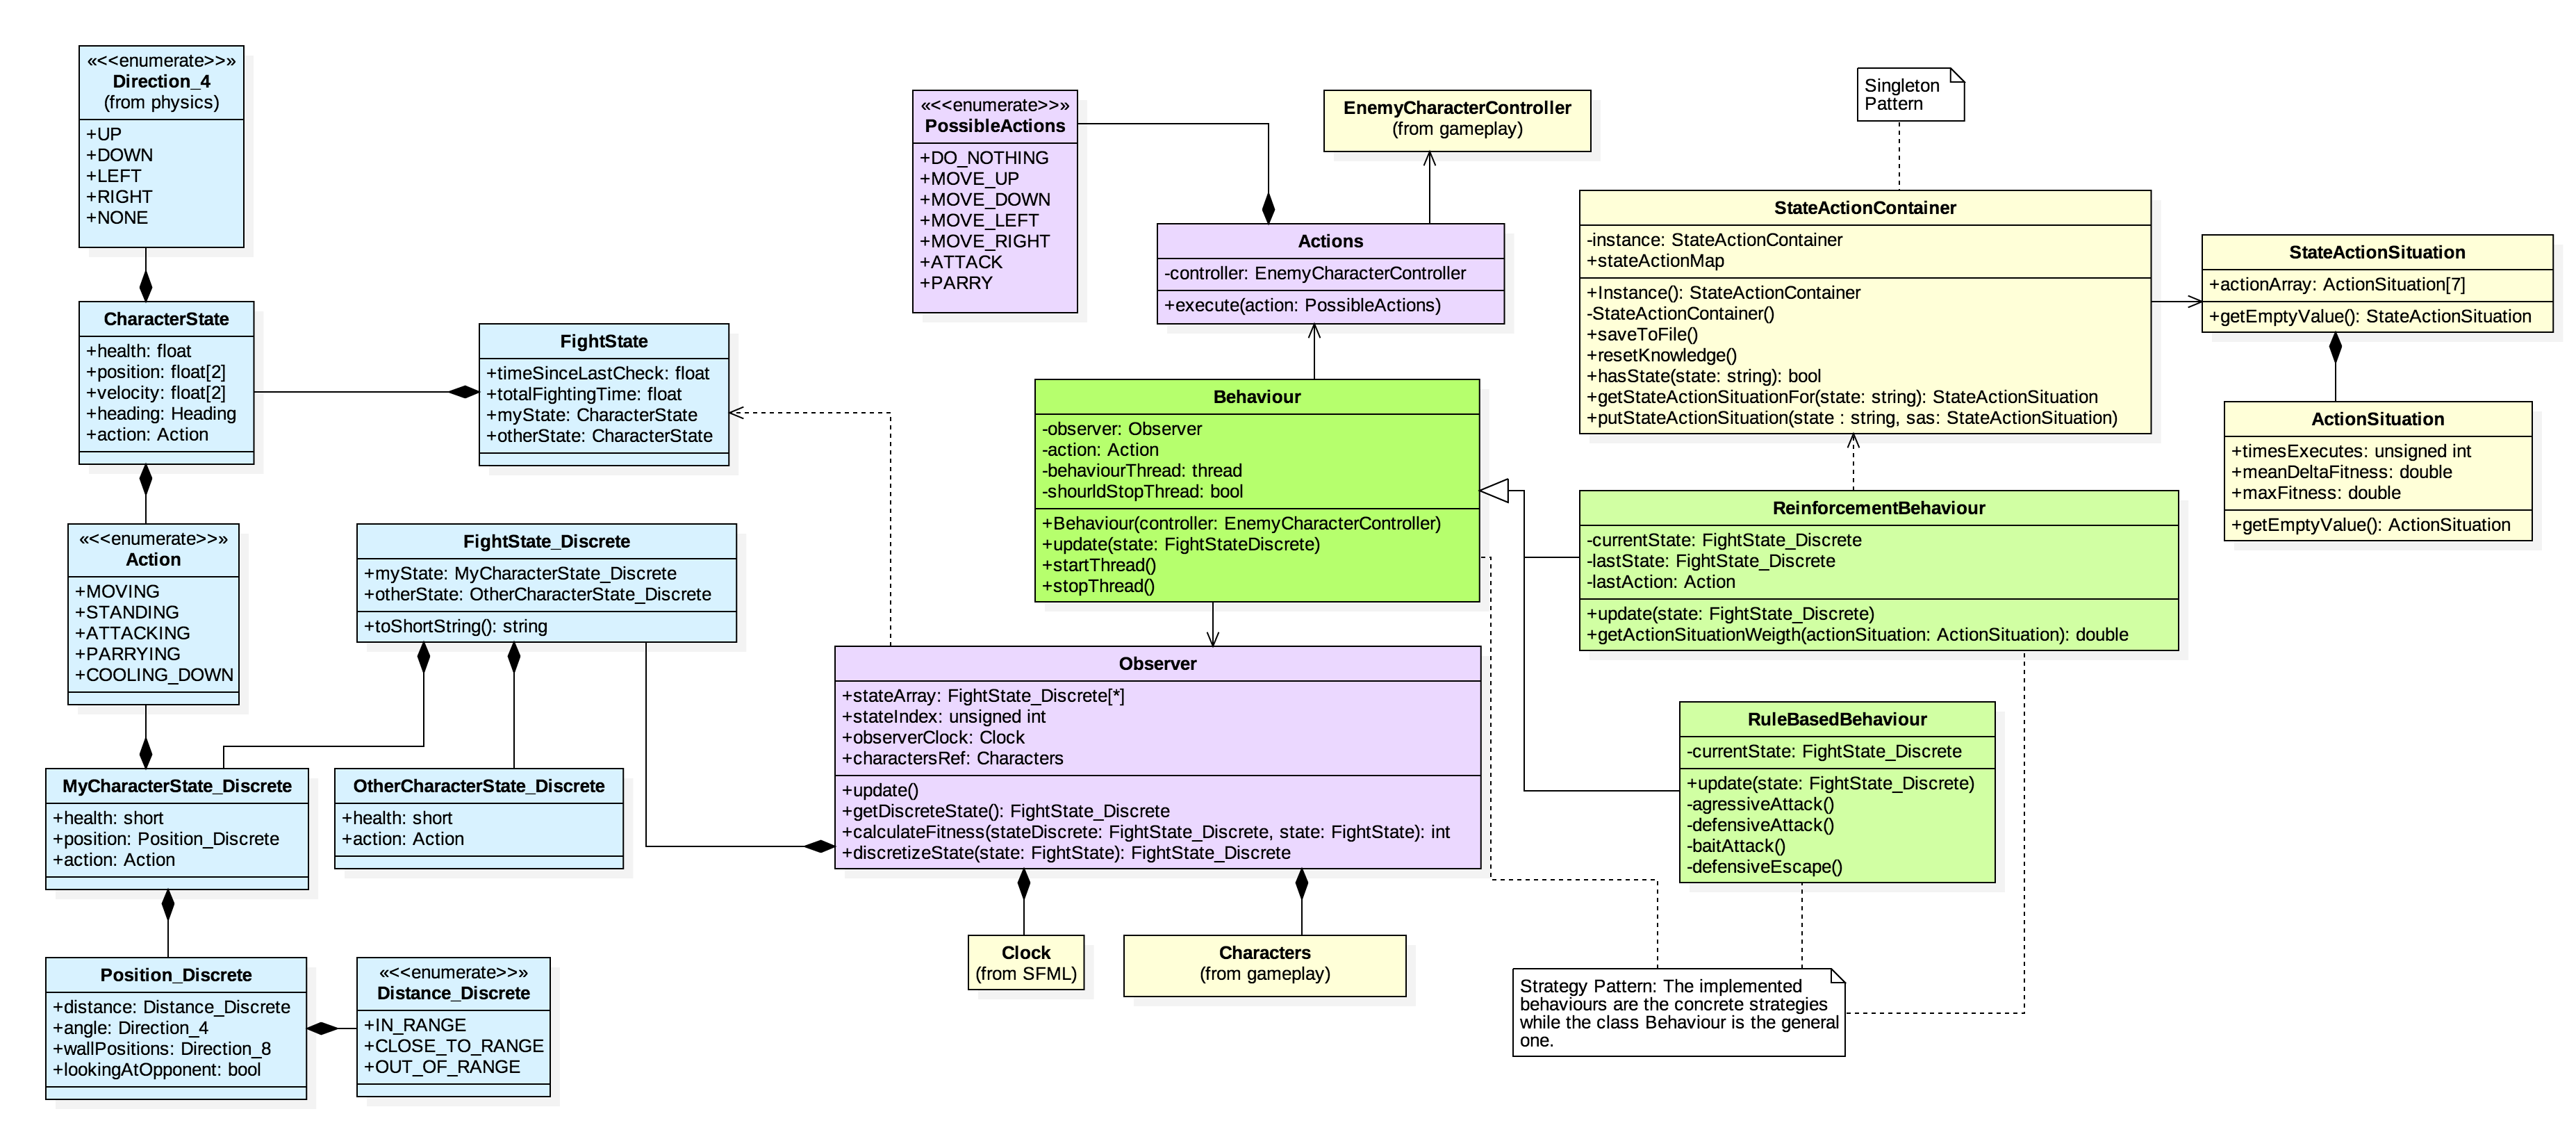
\includegraphics[width=24cm]{otros/UML/png/alld/png/gamelogic__gameplay__characterAI__diagramaDeClases_IA_5.png}
		\caption{Diagrama de clases del comportamiento del agente}
		\label{class:agent}
	\end{adjustwidth}
\end{figure}
\end{landscape}
\clearpage


\section{Diagramas de secuencia}

\begin{figure}
	\centerline{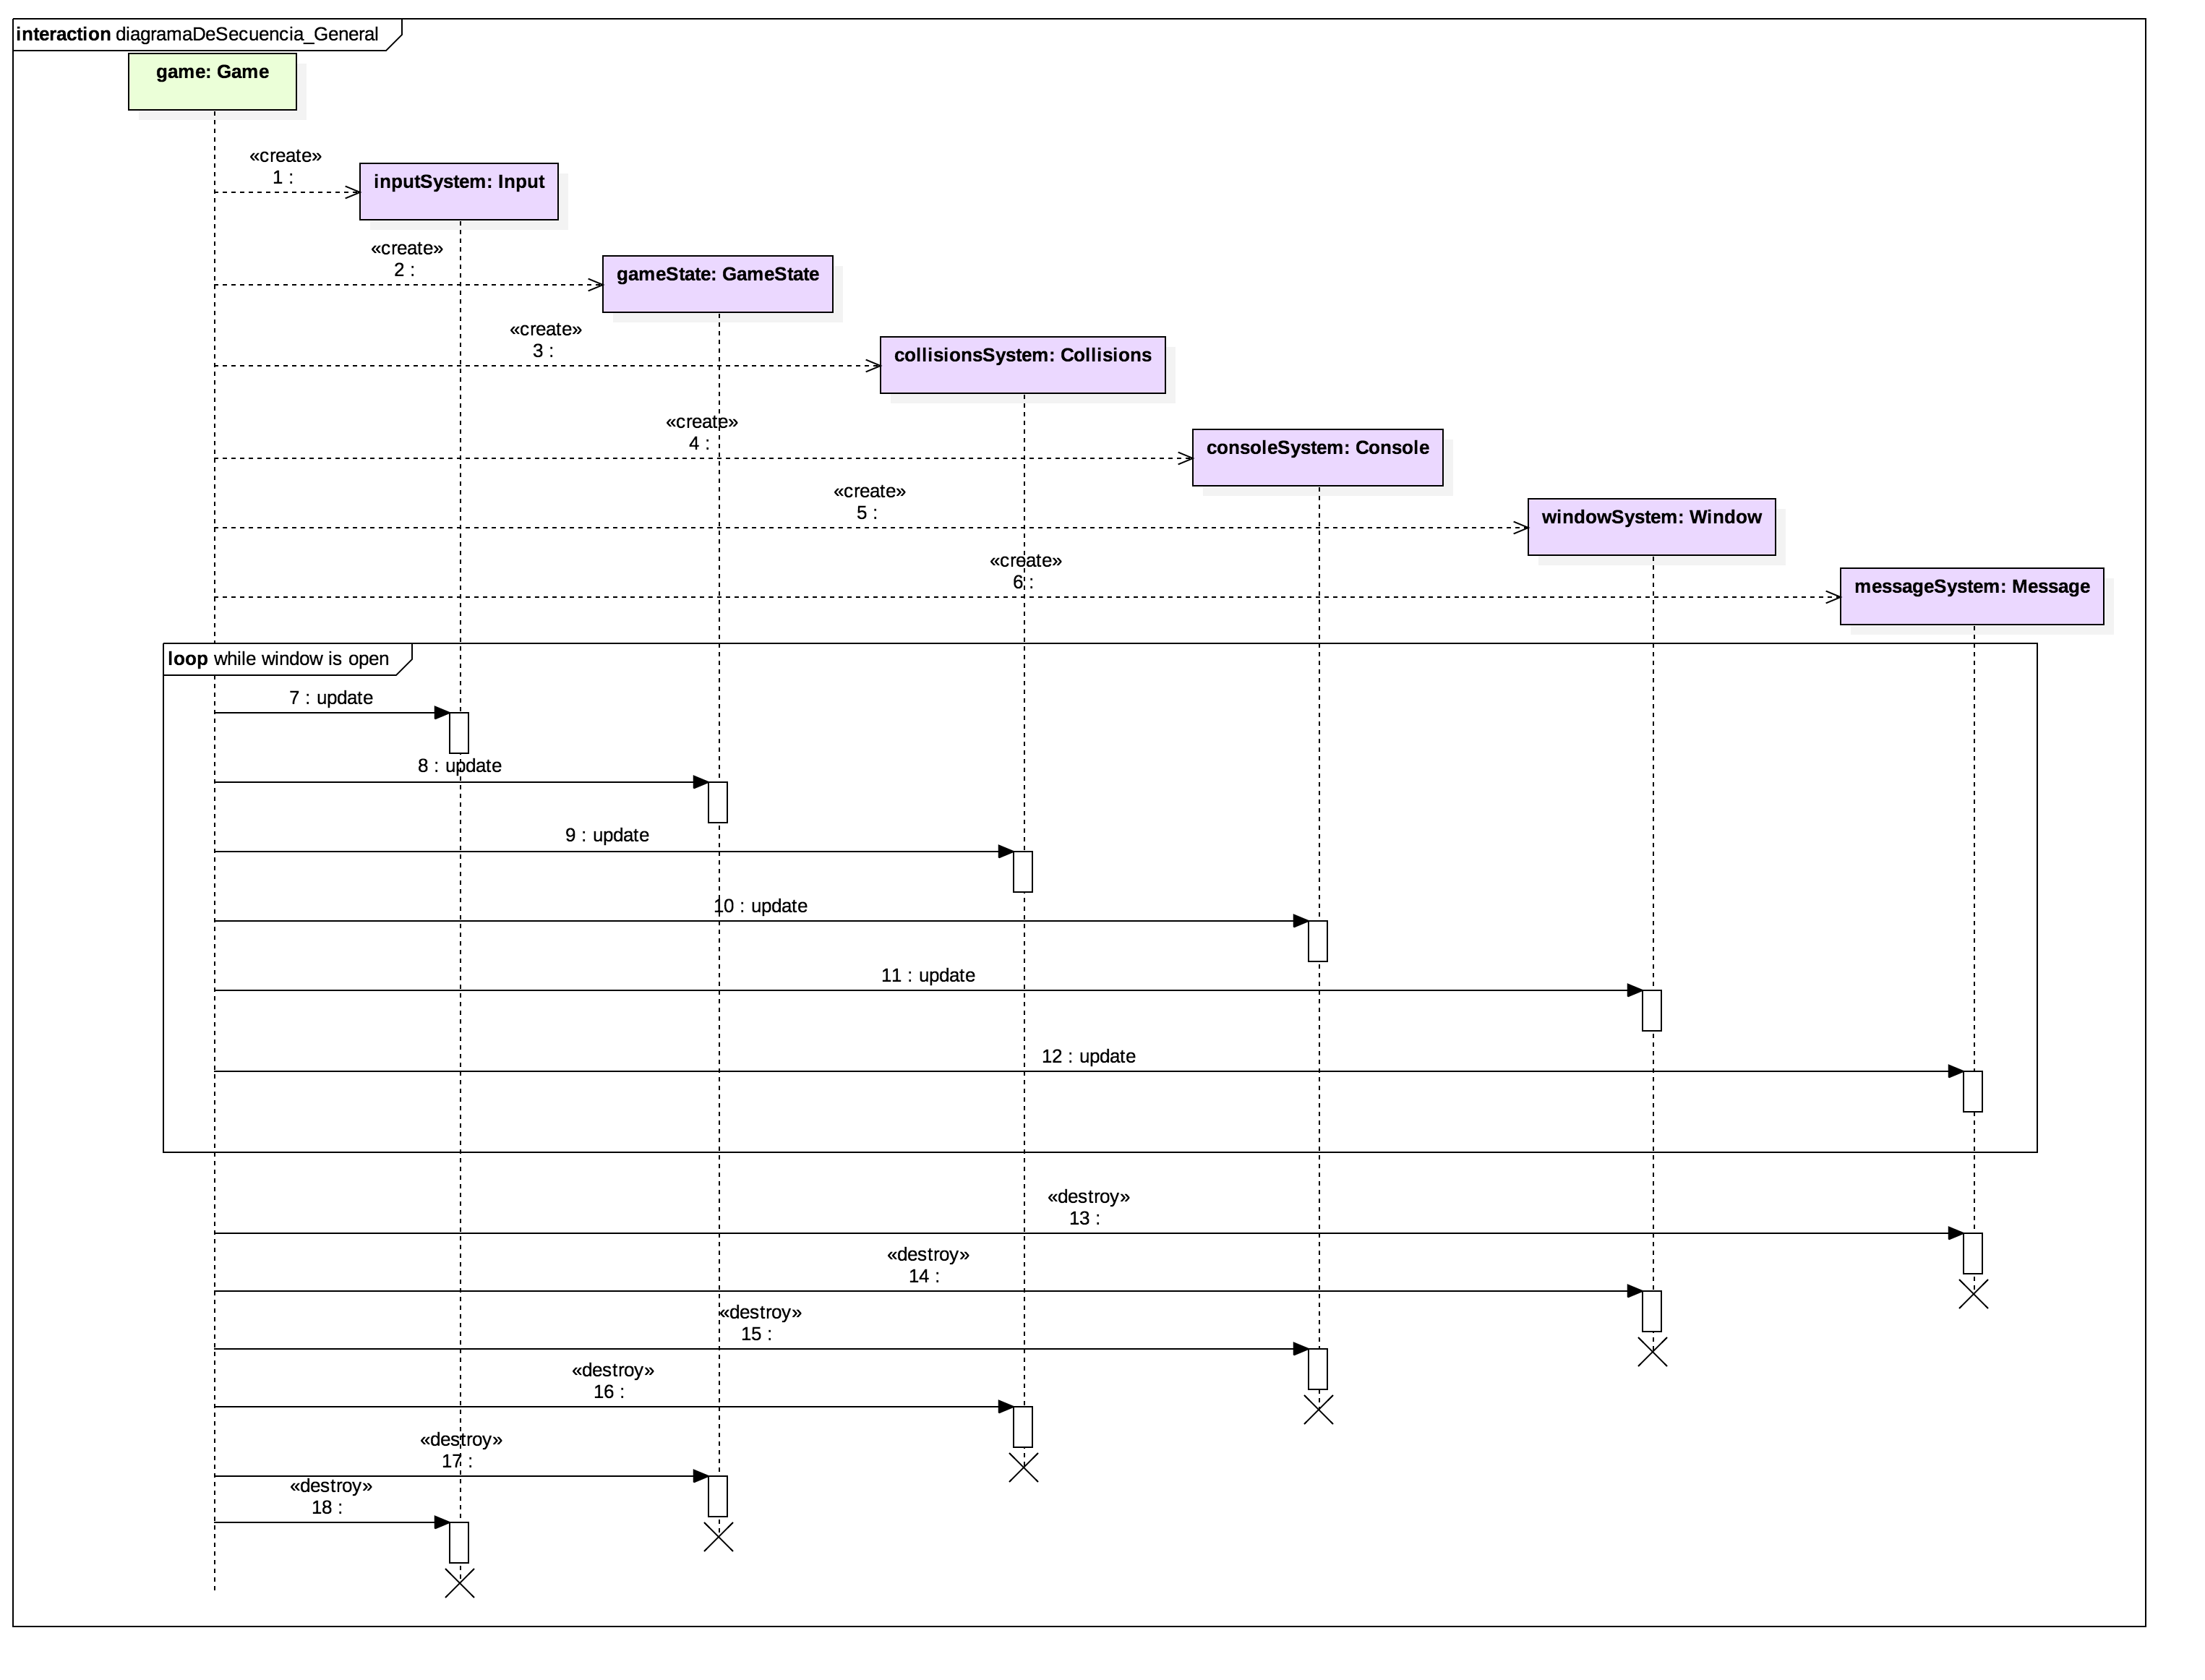
\includegraphics[width=19cm]{otros/UML/png/alld/png/CasosDeUso__General__Collaboration1__Interaction1__diagramaDeSecuencia_General_15.png}}
	\caption{Diagrama de secuencia general de la aplicación}
	\label{sec:general}
\end{figure}

\begin{figure}
	\centerline{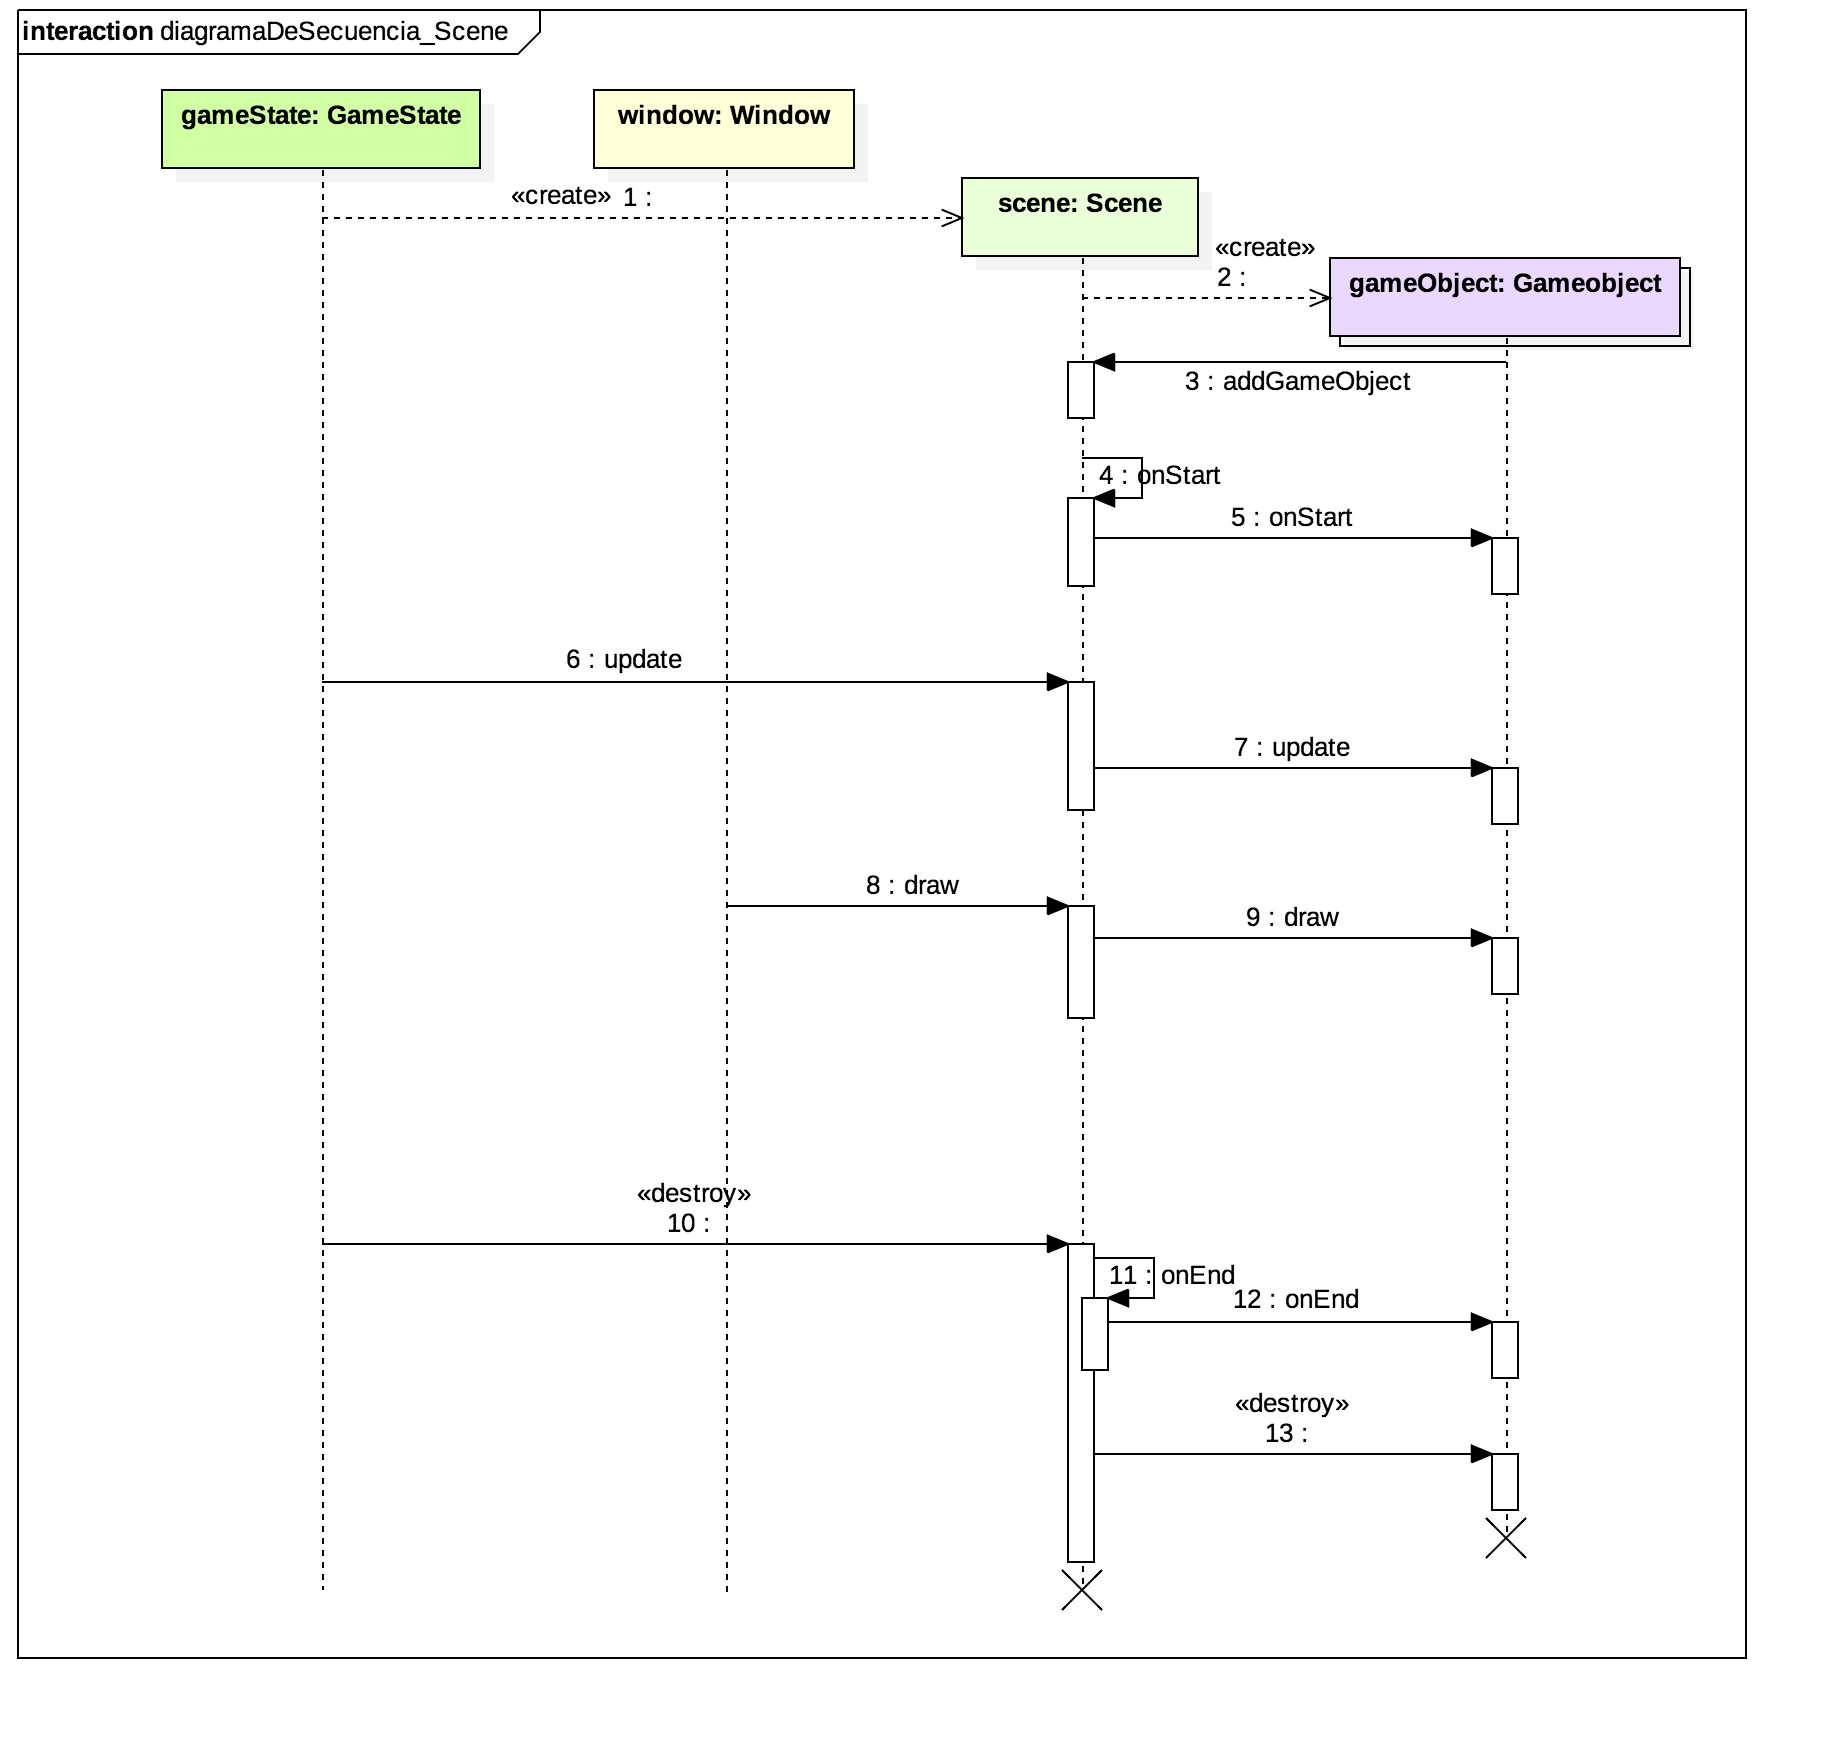
\includegraphics[width=15cm]{otros/UML/png/alld/png/CasosDeUso__General__Collaboration2__Interaction1__diagramaDeSecuencia_Scene_16.png}}
	\caption{Diagrama de secuencia genérico de una escena}
	\label{sec:scene}
\end{figure}

\begin{landscape}
\begin{figure}
	\hspace*{-3cm}  
	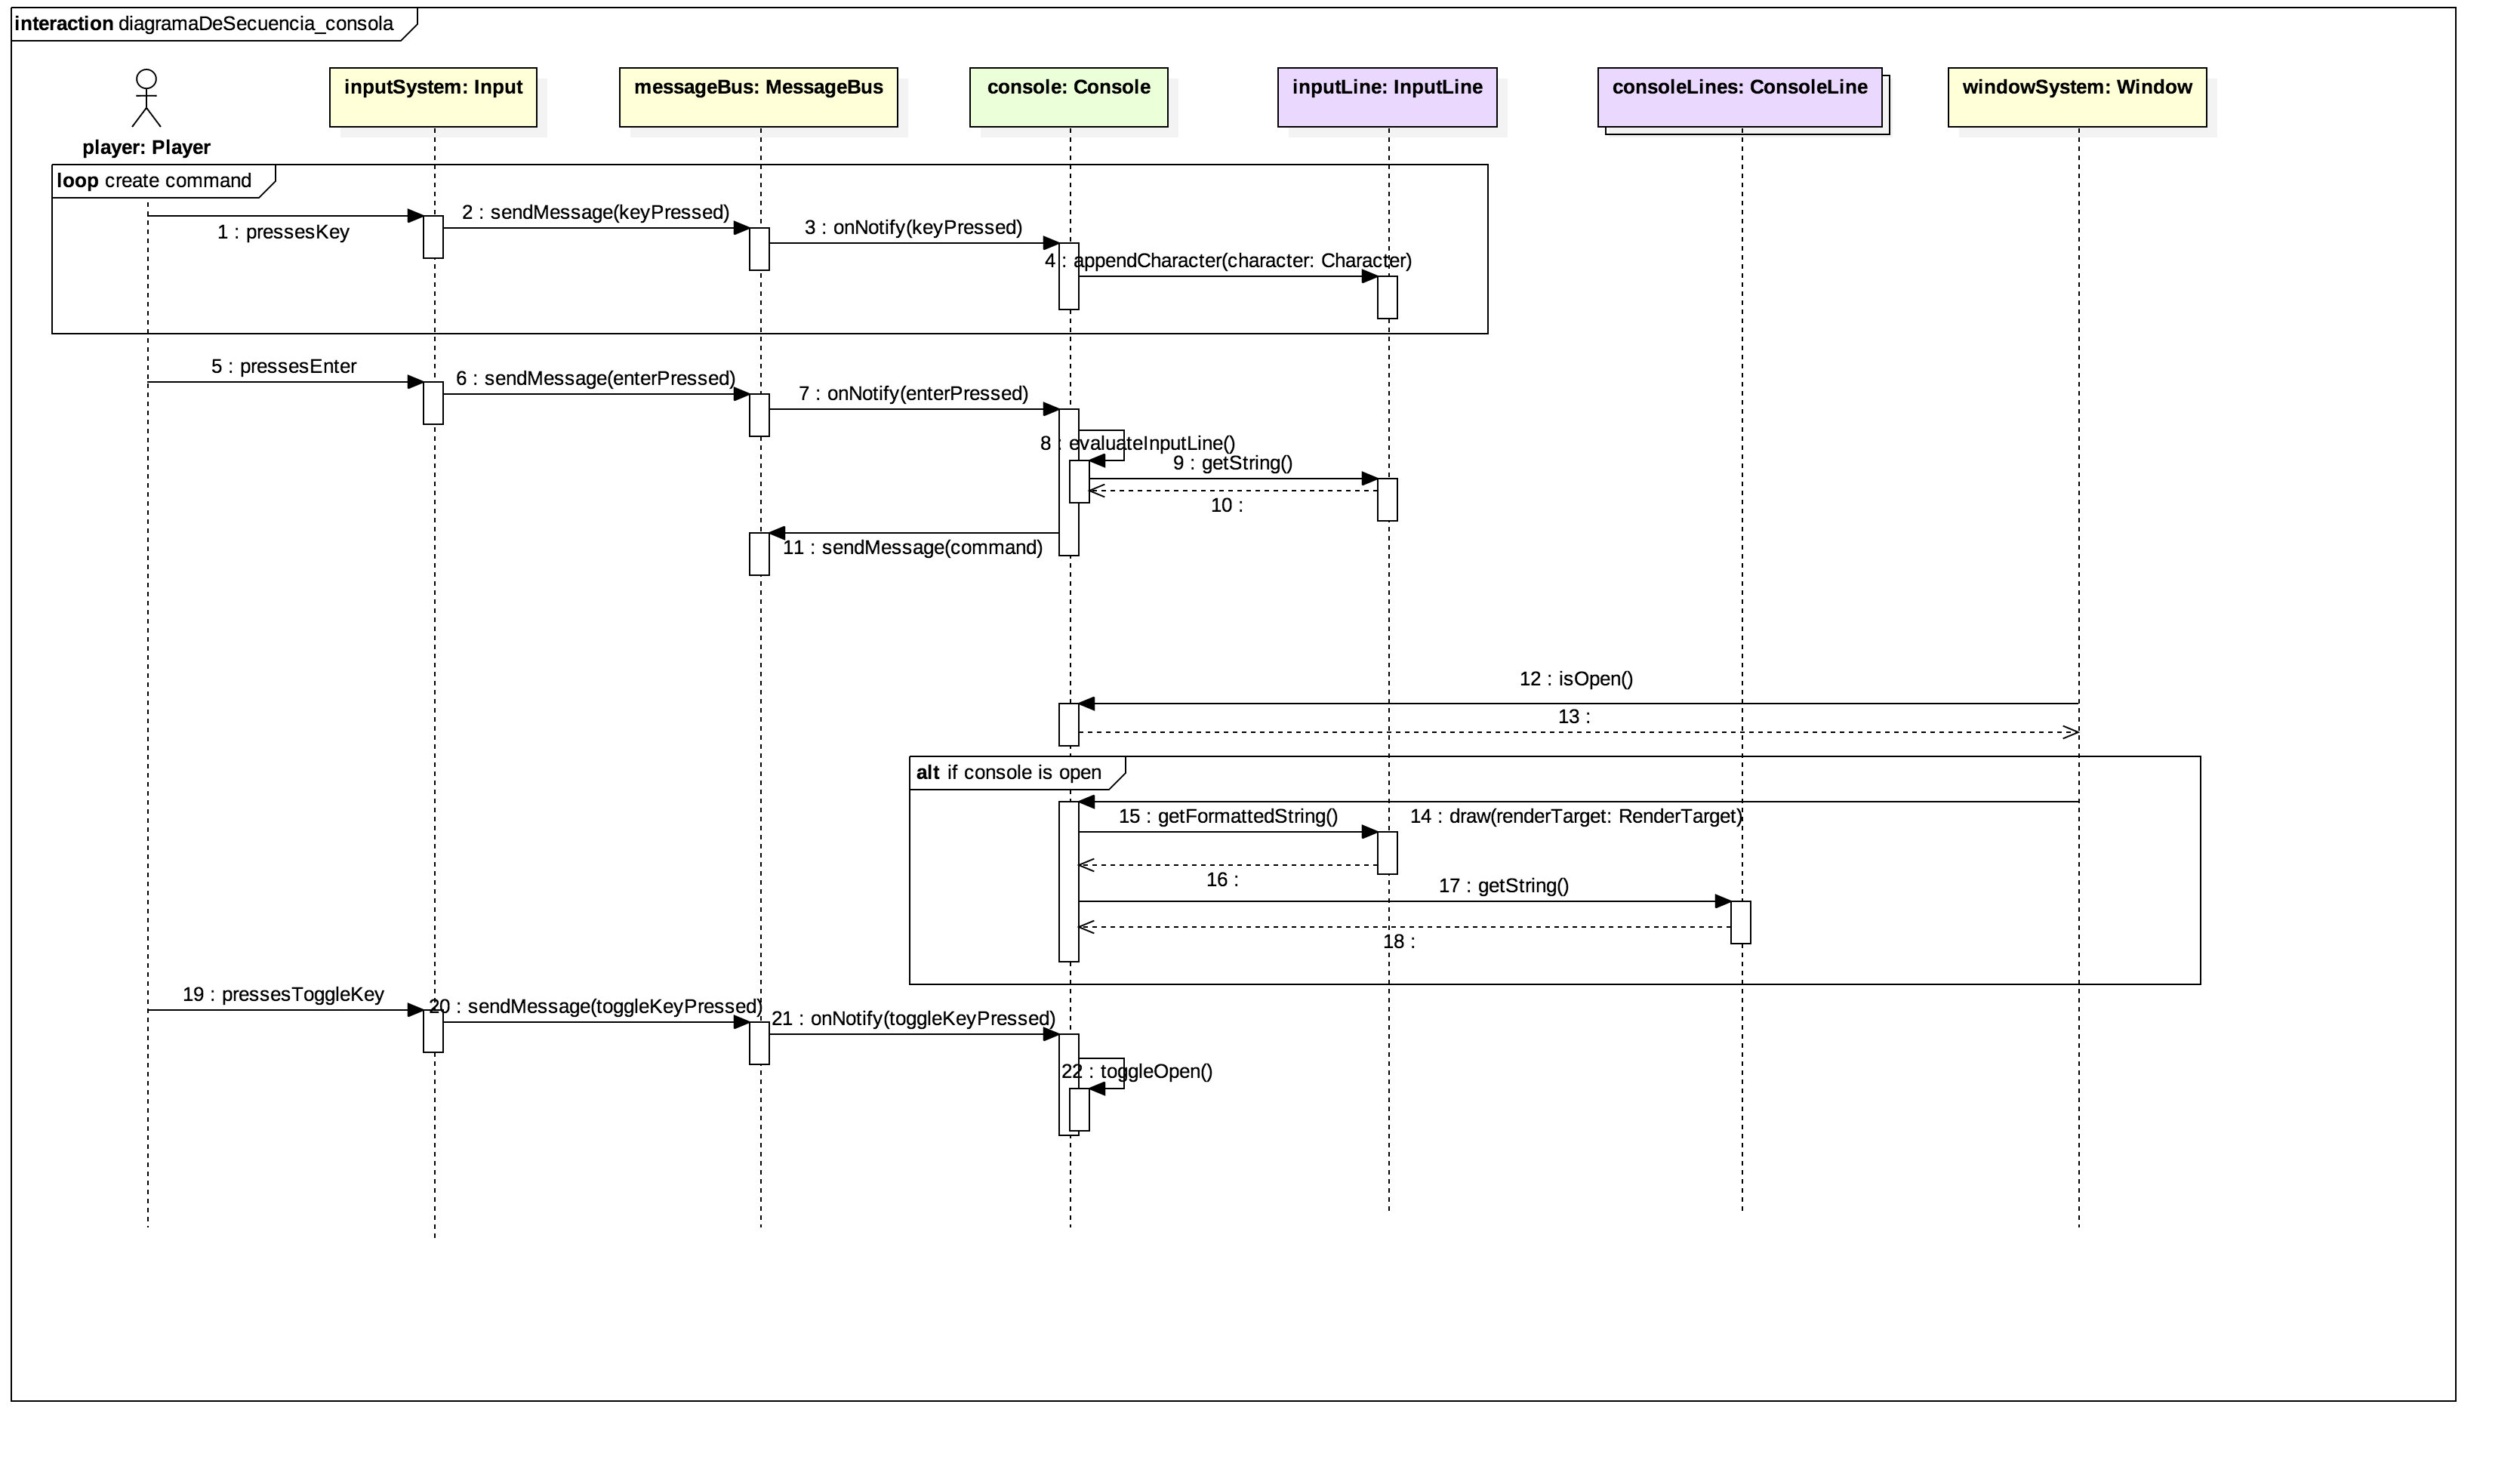
\includegraphics[width=24cm]{otros/UML/png/alld/png/CasosDeUso__Especifico__Collaboration4__Interaction1__diagramaDeSecuencia_consola_20.png}
	\caption{Diagrama de secuencia de la consola}
	\label{sec:console}

\end{figure}
\end{landscape}

\begin{landscape}
\begin{figure}
	\hspace*{-3cm}  
	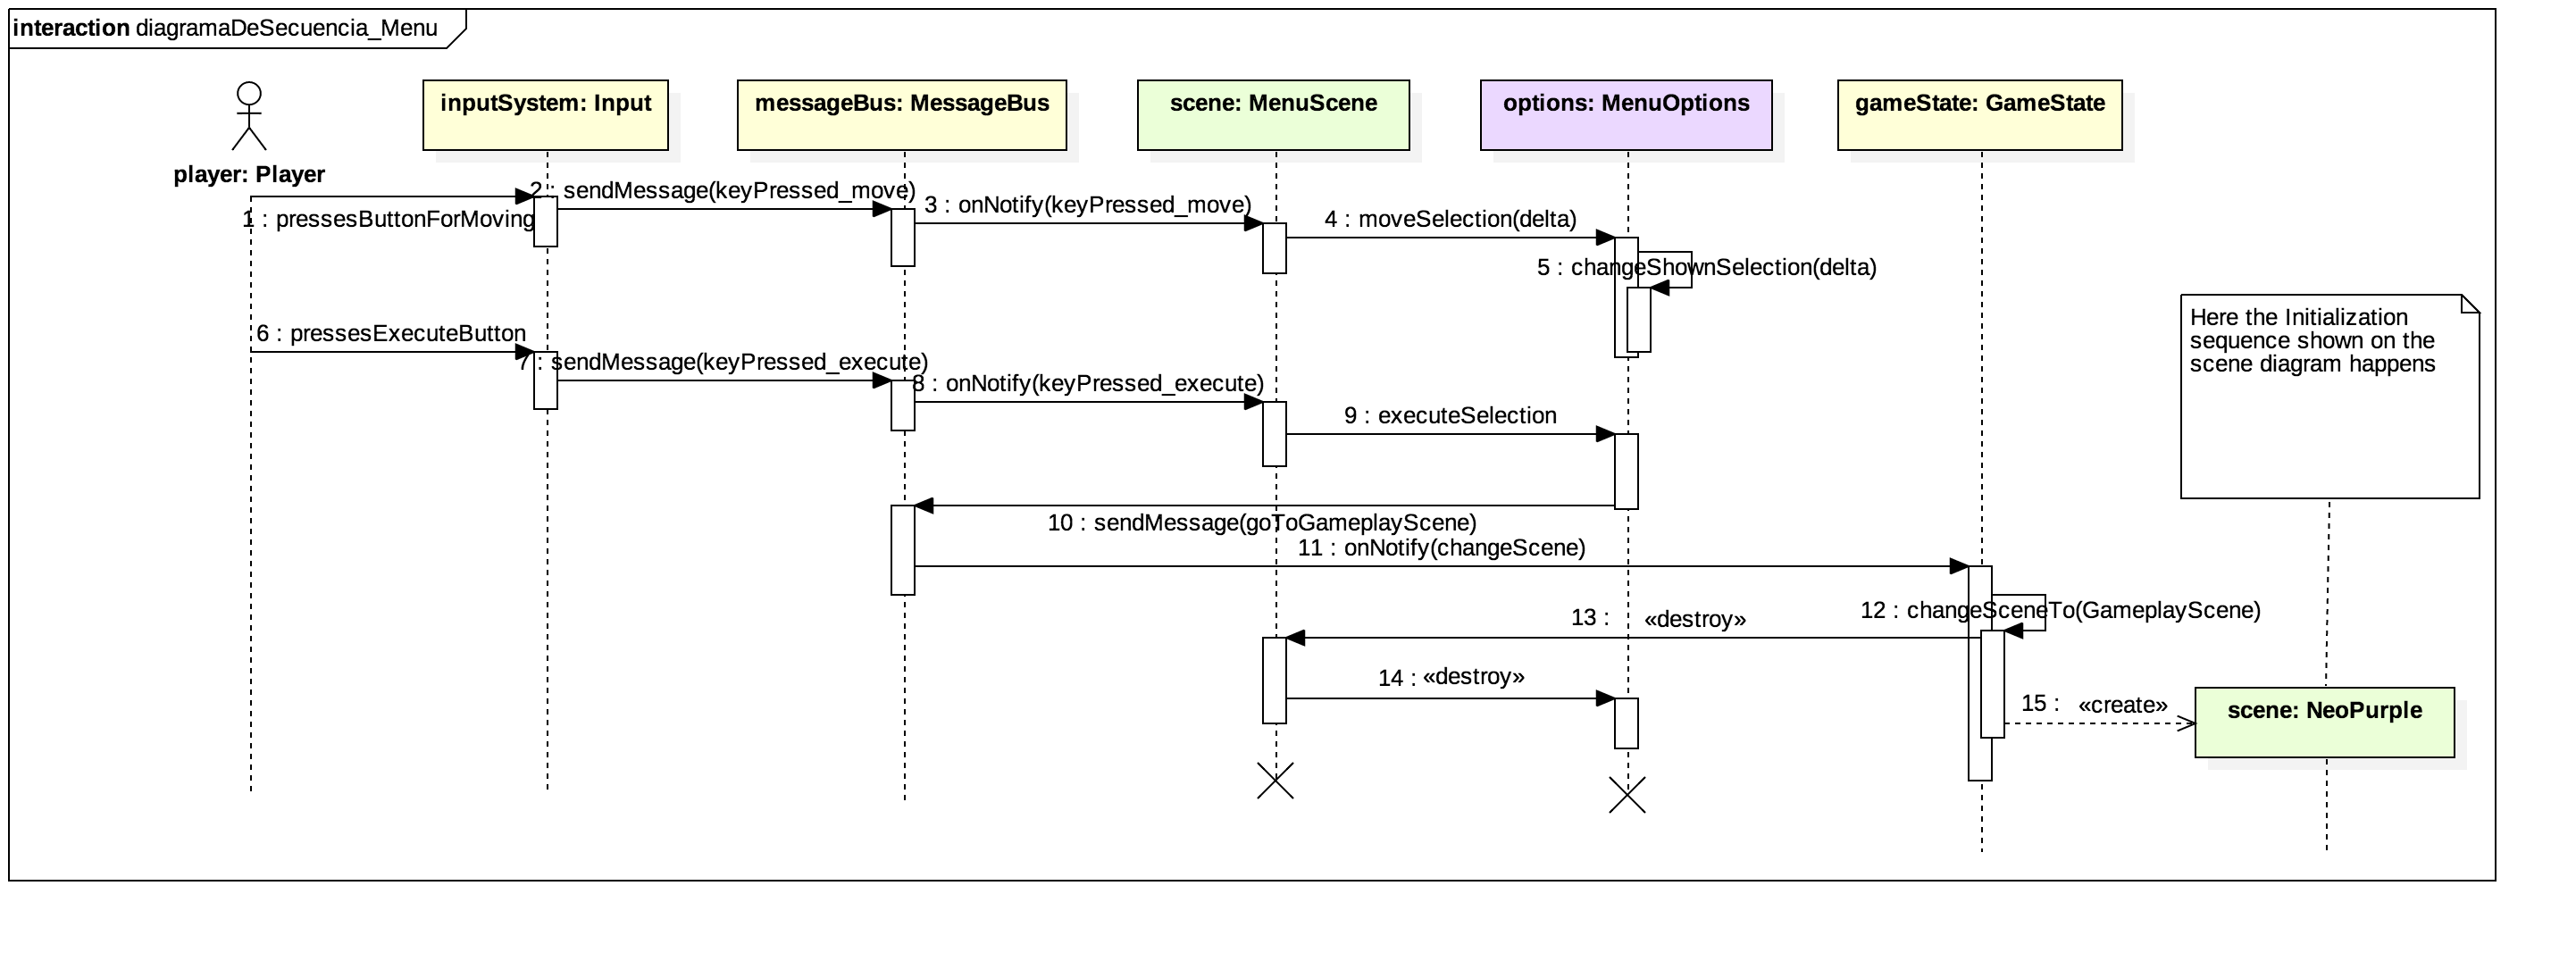
\includegraphics[width=24cm]{otros/UML/png/alld/png/CasosDeUso__Especifico__Collaboration1__Interaction1__diagramaDeSecuencia_Menu_17.png}
	\caption{Diagrama de secuencia de la escena del menú}
	\label{sec:menu}

\end{figure}
\end{landscape}

\begin{figure}
	\centerline{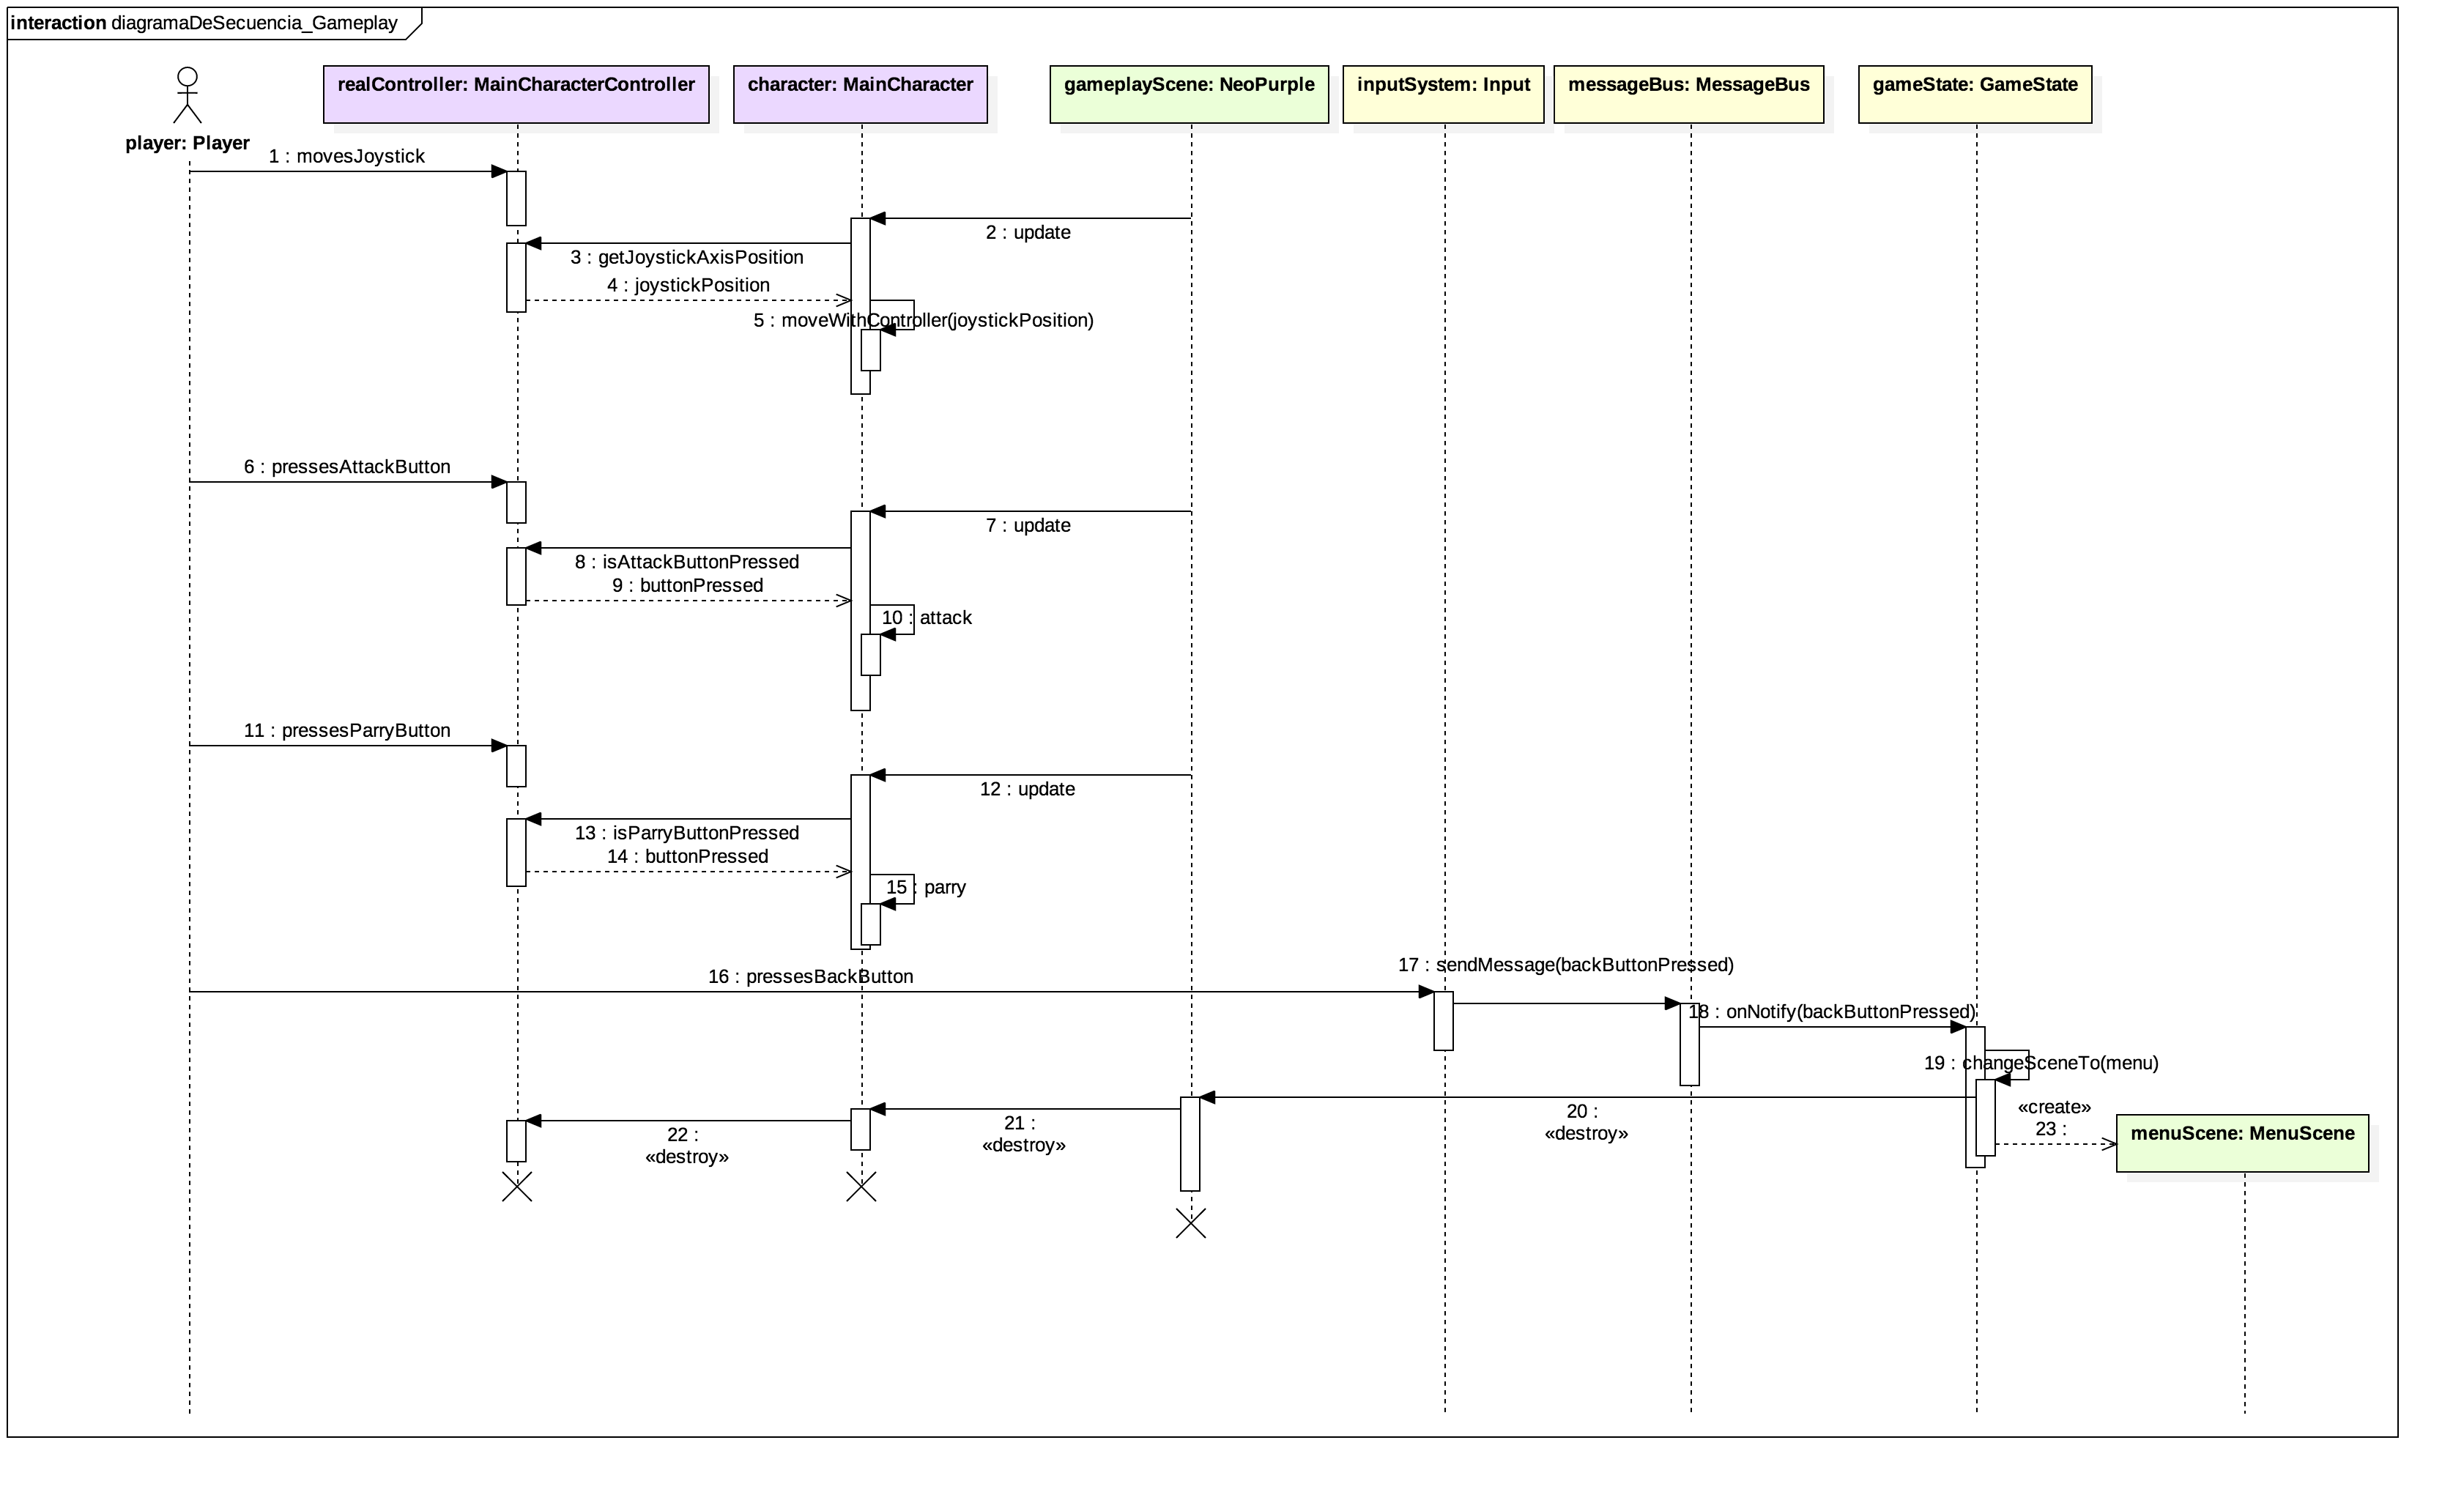
\includegraphics[width=19cm]{otros/UML/png/alld/png/CasosDeUso__Especifico__Collaboration2__Interaction1__diagramaDeSecuencia_Gameplay_18.png}}
	\caption{Diagrama de secuencia de la escena del \textit{gameplay}}
	\label{sec:gameplay}
\end{figure}

\begin{figure}
	\centerline{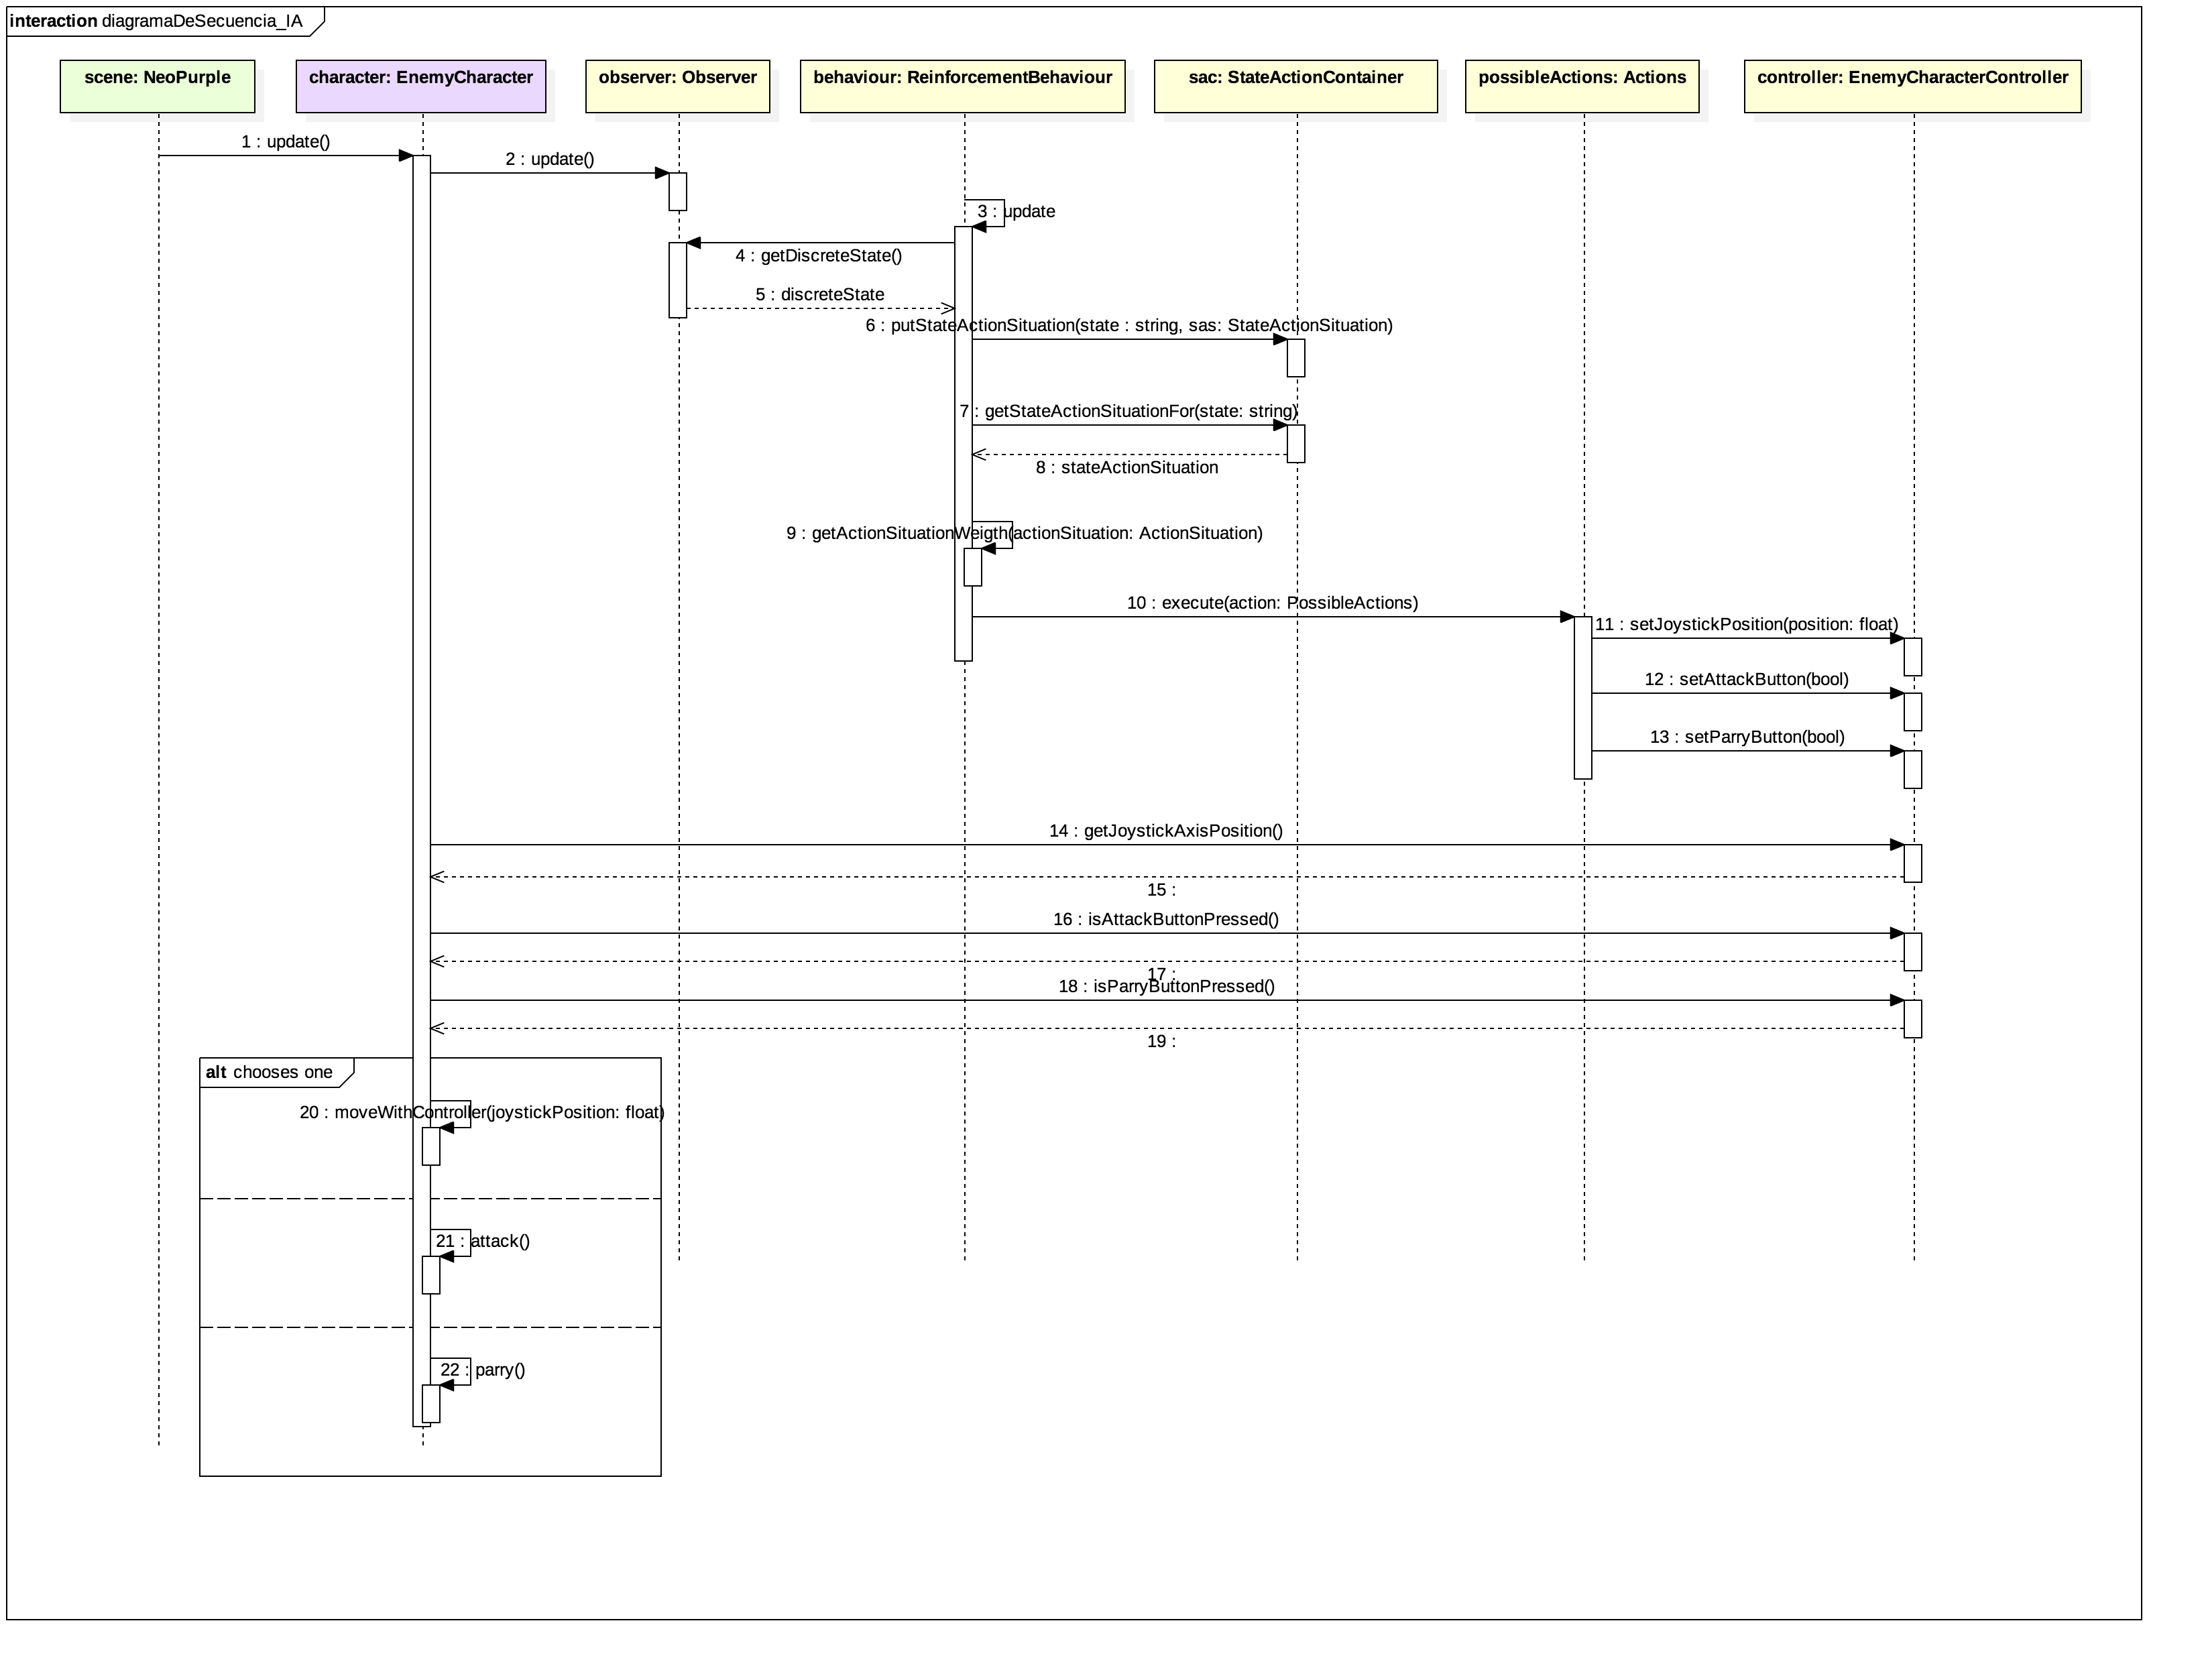
\includegraphics[width=19cm]{otros/UML/png/alld/png/CasosDeUso__Especifico__Collaboration3__Interaction1__diagramaDeSecuencia_IA_19.png}}
	\caption{Diagrama de secuencia del agente}
	\label{sec:agent}
\end{figure}

